\documentclass[11pt]{article}
% Single-column layout matching Word document style
\usepackage[a4paper, margin=2.5cm]{geometry}
% Use ACL bibliography style only (not the two-column layout)
\usepackage{natbib}
\bibliographystyle{acl_natbib}
\usepackage{times}
\usepackage{latexsym}
\usepackage[T1]{fontenc}
\usepackage[utf8]{inputenc}
\usepackage{microtype}
\usepackage{graphicx}
\usepackage{booktabs}
\usepackage{multirow}
\usepackage{amsmath}
\usepackage{url}
% Load hyperref but disable all link colouring
\usepackage[hidelinks]{hyperref}
\usepackage{float}          % provides [H] specifier to force float placement
\usepackage{parskip}        % paragraph spacing instead of indent
\usepackage{setspace}
\setstretch{1.15}           % comfortable line spacing

\title{Decoupling Urgency and Emotion in Automated\\Telecom Complaint Triage}
\date{}

\author{
  \textbf{Liqiang Cheng} (25078815) \quad
  \textbf{Olena Brylinska} (25190473) \quad
  \textbf{Yuansheng Tao} (25155204) \\[2pt]
  \textbf{Yuyi Song} (25206842) \quad
  \textbf{Yuzhi Zhao} (25172008) \\[4pt]
  UCL School of Management, University College London \\
  MSIN0221 Group Assignment --- Group 16 \\
  31 March 2026
}

\begin{document}
\maketitle

% ── Abstract ─────────────────────────────────────────────────────────────────
\begin{abstract}
Automated complaint triage in telecommunications requires two simultaneous
judgements: how operationally severe is the underlying issue, and how
emotionally escalated is the customer? These dimensions are conceptually
orthogonal yet are routinely conflated by existing prioritisation systems.
This paper introduces a 5,000-complaint synthetic UK telecoms dataset with
independently controlled urgency and emotion labels across a $3{\times}3$
grid, and evaluates four classification architectures: few-shot Claude Haiku~4.5,
TF-IDF + Logistic Regression, frozen Sentence-BERT + Logistic Regression, and
fine-tuned DeBERTa-v3-base with dual classification heads. DeBERTa achieves
the strongest combined performance (macro F1 = 0.830), with a particularly
clear advantage on emotion classification (0.857 vs.\ 0.764 for TF-IDF).
An 18.6 percentage-point gain in urgency F1 from dataset v2 to v3 demonstrates
that generation quality was the primary bottleneck. Contrastive error analysis
using Informative Correct Pairs identifies recurring blind spots in both heads,
validated through targeted adversarial stress testing.
\end{abstract}

% ── Word count (main body, excluding abstract, appendices, references, captions) ──
\noindent\textbf{Word count:} 3,885

% ── Member Contribution Breakdown ────────────────────────────────────────────
\vspace{0.3em}
\noindent\textbf{Team Contributions}

\vspace{0.2em}
\noindent\small
\begin{tabular}{@{}clp{8.0cm}p{4.2cm}@{}}
  \toprule
  \textbf{\#} & \textbf{Name} & \textbf{Actual Contributions} & \textbf{Report Section} \\
  \midrule
  1 & Liqiang Cheng   & Introduction, Literature Review, Research Framework Design, Error Analysis (co-lead) & Section 1: Introduction \& Literature Review; Section 5 \\
  \addlinespace
  2 & Yuansheng Tao   & Synthetic Dataset Design (v1--v3), DeBERTa Architecture \& Training (Runs 1--8) & Section 2: Data; Section 3: Methodology \\
  \addlinespace
  3 & Yuzhi Zhao      & EDA, TF-IDF / SBERT / Haiku Baselines, Model Comparison \& Evaluation & Section 4: Results \& Evaluation \\
  \addlinespace
  4 & Olena Brylinska & Contrastive Error Analysis (co-lead), Blindspot Taxonomy, Adversarial Testing, Limitations & Section 5: Error Analysis \& Discussion \\
  \addlinespace
  5 & Yuyi Song       & Conclusion, Business Application, Report Integration \& Presentation & Section 6: Conclusions \\
  \bottomrule
\end{tabular}\normalsize

% ─────────────────────────────────────────────────────────────────────────────
\section{Introduction}
% ─────────────────────────────────────────────────────────────────────────────

Customer-facing complaint handling in the telecommunications sector presents a
triage challenge that is difficult to automate. When a support agent receives an
inbound complaint, they must make two simultaneous judgements: how objectively serious
is the underlying issue, and how emotionally escalated is the customer expressing that
issue? These are not the same questions. A customer who writes \textit{``I would like
to \textbf{flag}, at your earliest convenience, that our office has had no
\textbf{connectivity} for seventy-two hours and we are losing approximately three
thousand pounds per day''} is describing a catastrophic situation in perfectly calm
prose. A customer who writes \textit{``THIS IS ABSOLUTELY DISGUSTING I CANNOT BELIEVE
YOU CHANGED THE APP FONT''} is emotionally escalated about something trivial.
Misrouting these two cases is precisely the failure mode that automated triage must
avoid. Research also shows that even the best available language models often mix up
closely related emotion categories when they have not been fine-tuned for the specific
domain \citep{zhang2024sentiment}.

The case for automating complaint triage with NLP is well established.
\citet{vairetti2024} demonstrate that transformer-based deep learning models can
automatically label and prioritise large volumes of complaints with high accuracy,
achieving 92.1\% accuracy on over 44,000 complaints using a BERT-based architecture
combined with multicriteria decision-making. More recently, \citet{roumeliotis2025}
evaluated fourteen LLMs on zero-shot consumer complaint classification, finding that
while reasoning models offer improved contextual understanding, they incur
significantly higher processing time and inference cost compared to fine-tuned
specialist models. A related challenge concerns the availability of labelled training data for such tasks.
\citet{long2024llms} propose a generic framework for LLM-based
synthetic dataset generation, demonstrating that LLMs can produce diverse,
task-relevant training examples at low cost. However, \citet{tan2024annotation} caution
that LLM-generated annotations carry inherent quality risks, including label--text
deception, where the generated label does not truthfully reflect the content of the
generated text, a limitation that motivates careful quality control in any synthetically
labelled pipeline.

A key gap in existing literature motivates the present work. Existing complaint
prioritisation frameworks treat urgency as a composite label that conflates objective
issue severity with the emotional tone of the customer.
\citet{athira2025} find that different model architectures perform best on different
complaint analysis dimensions, with no single architecture achieving uniform high
performance across sentiment, emotion, and severity simultaneously. Their finding
suggests that these dimensions require distinct modelling approaches rather than
treatment as a unified composite label.

Against this background, this paper asks: \textit{How effectively can different NLP
models classify urgency and emotional intensity independently in synthetic UK telecom
complaints, and what error patterns emerge when these dimensions are disentangled by
design?}

This paper presents three contributions that directly address this gap. First, we
introduce a 5,000-complaint synthetic dataset of UK telecoms complaints with
fine-grained orthogonal control over four dimensions: scenario, writing style, customer
profile, and complaint history, in which urgency and emotional intensity are deliberately
decoupled by design. Second, we fine-tune a DeBERTa-v3-base model for dual-head
classification and compare it against three baselines: TF-IDF with Logistic Regression,
frozen Sentence-BERT with Logistic Regression, and few-shot Claude Haiku~4.5. Third, we
conduct a per-instance causal error analysis augmented by Informative Correct Predictions
(ICP), adapted from \citet{ashuryTahan2026}, by matching incorrect and correct
predictions that share metadata in order to identify the linguistic patterns responsible
for model failure.

% ─────────────────────────────────────────────────────────────────────────────
\section{Data}
% ─────────────────────────────────────────────────────────────────────────────

\subsection{Why Synthetic Data}

No publicly available dataset provides dual ground-truth labels for both urgency and
emotional intensity in customer complaints. Existing open complaint corpora, such as the
Consumer Financial Protection Bureau dataset, are either unlabelled on these dimensions,
domain-mismatched, or annotated for a single dimension only. The two dimensions are
seldom framed as independent classification targets in publicly available resources.
Real-world telecoms complaints additionally carry privacy constraints that limit
redistribution. Generating synthetic data allowed us to guarantee label correctness by
design: rather than annotating text post-hoc and reconciling inter-annotator
disagreement, we instructed the generation model to write each complaint to a specified
urgency and emotion level, making the intended label the ground truth by construction.

\subsection{Dataset Design and Generation}

The dataset consists of 5,000 complaints structured as a $3{\times}3$ grid, with
urgency on one axis and emotion on the other. The urgency distribution reflects a
realistic skew where critical operational contacts are assumed to be less frequent than
routine ones. Emotion is distributed evenly within each urgency group. The dataset is
split 70/15/15 into training (3,500), validation (750), and test (750) sets, stratified
on the full urgency-by-emotion cell to preserve the intended class distribution across
all three partitions.

\begin{figure}[H]
  \centering
  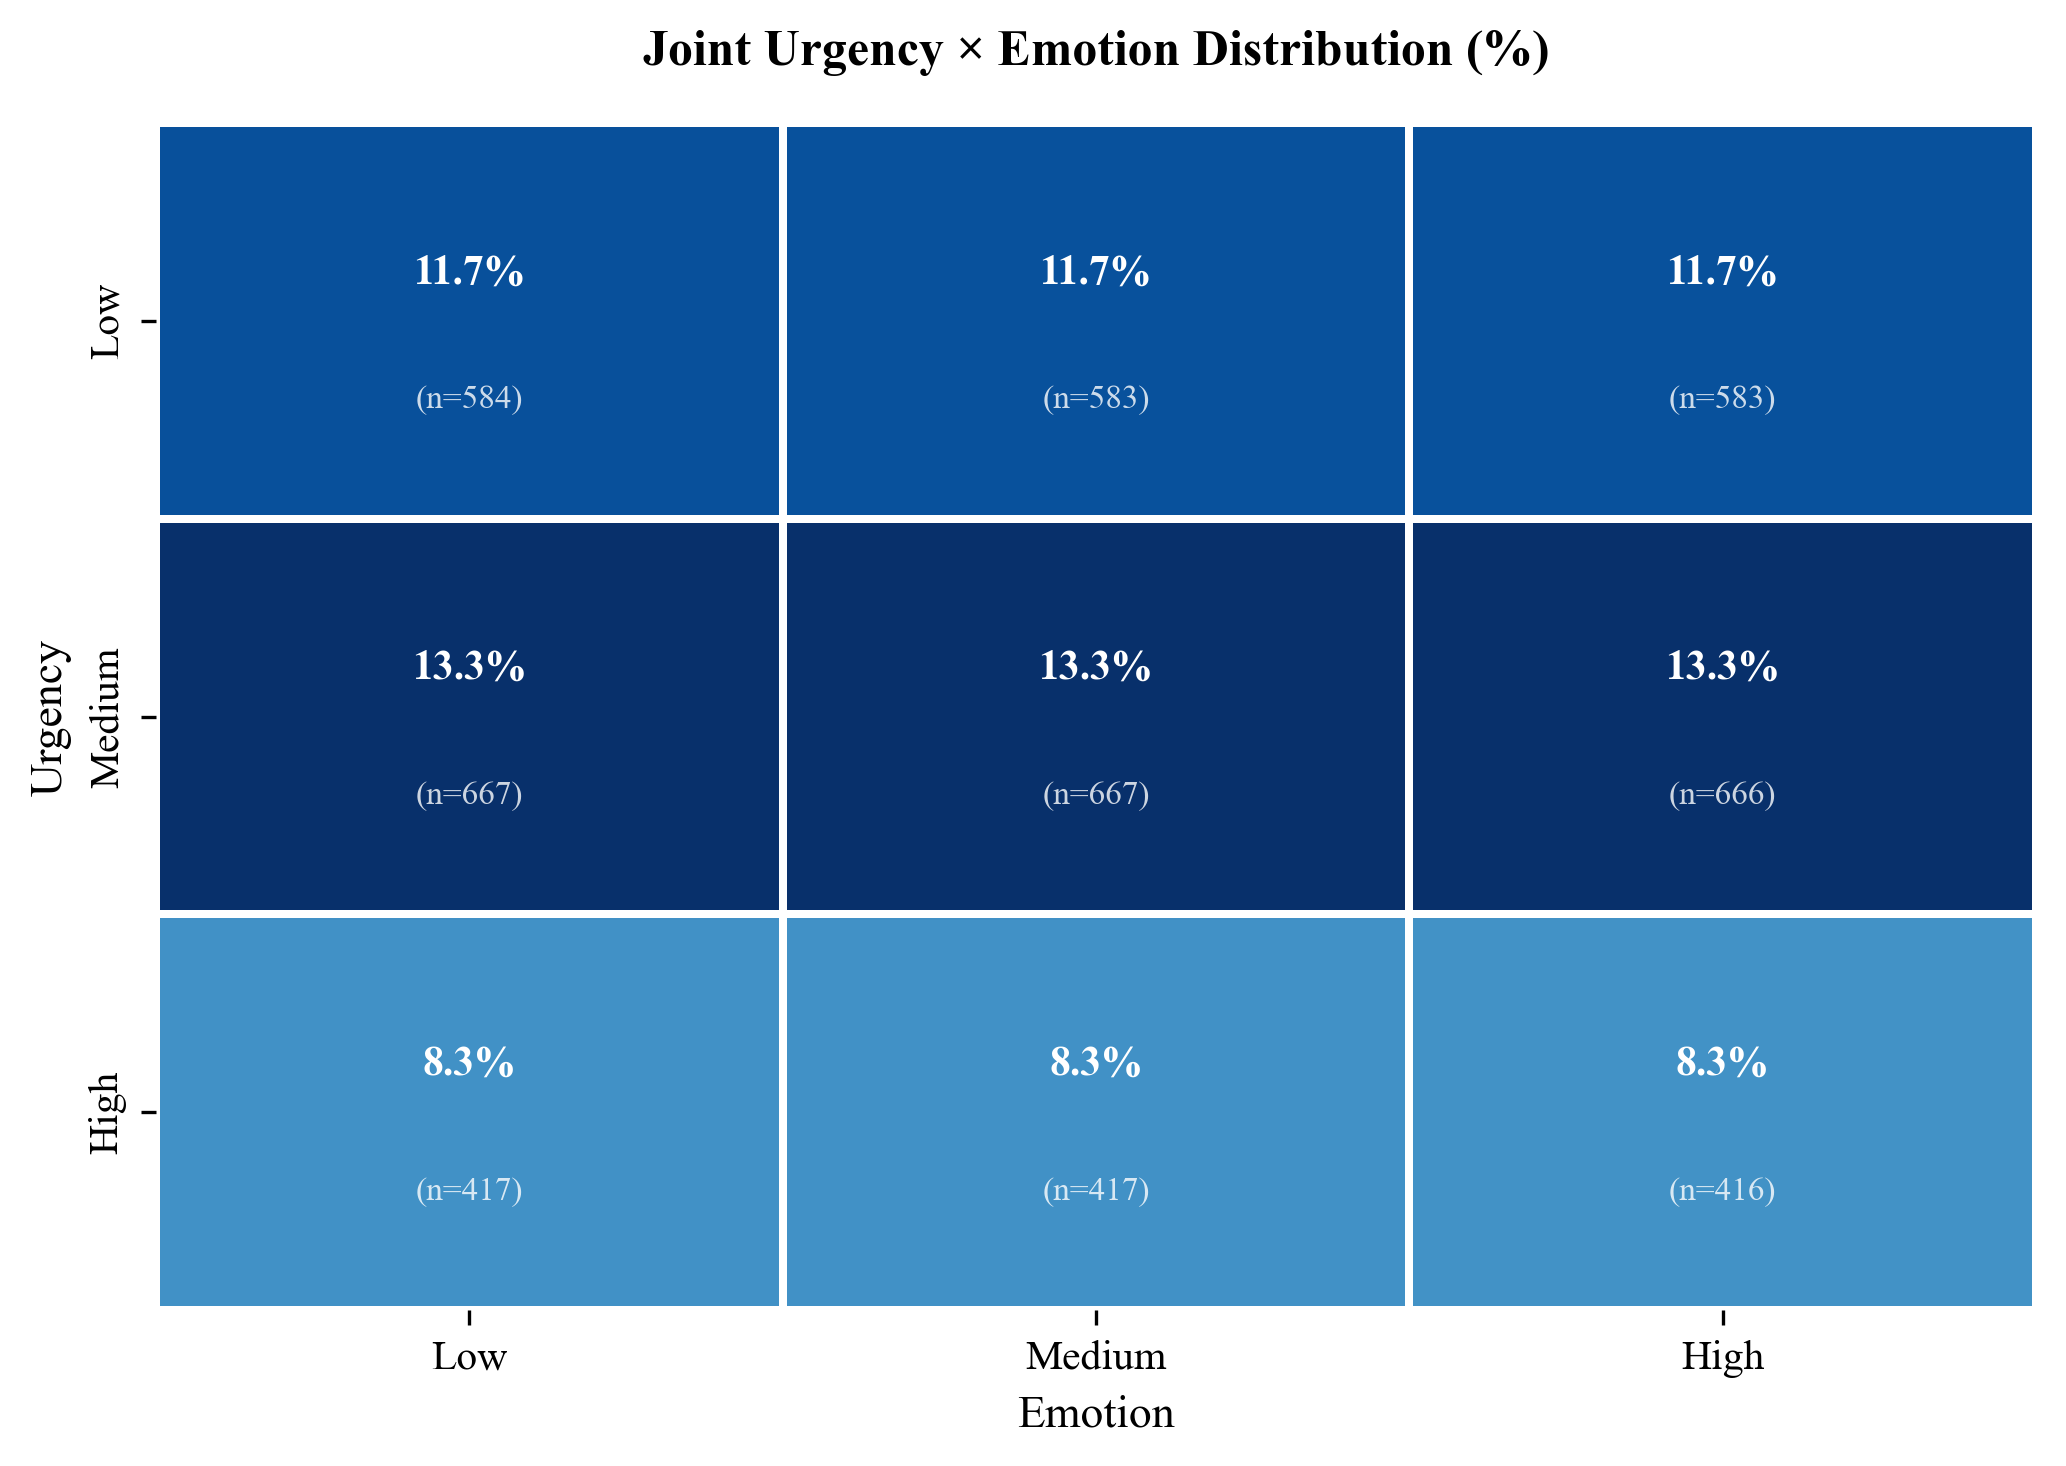
\includegraphics[width=0.75\columnwidth]{figures/fig01_joint_distribution.png}
  \caption{Joint urgency $\times$ emotion distribution (\%) across the 5,000-complaint
  synthetic dataset.}
  \label{fig:joint}
\end{figure}

Each complaint is assigned four characteristics prior to generation, ensuring
linguistic diversity within and across cells (Table~\ref{tab:creation_rules}).

\begin{table}[H]
  \centering
  \small
  \begin{tabular}{lp{3.5cm}p{2.8cm}}
    \toprule
    \textbf{Dimension} & \textbf{Options} & \textbf{Purpose} \\
    \midrule
    Scenario        & 20 UK telecoms topics & Controls subject matter \\
    Writing style   & 8 styles (e.g.\ formal, sarcastic, legalistic) & Controls surface-level form \\
    Customer profile & 8 personas (e.g.\ elderly, small business) & Controls voice and framing \\
    Complaint history & 4 depths (first contact to escalation) & Controls implied severity context \\
    \bottomrule
  \end{tabular}
  \caption{Synthetic data creation rules: the four characteristics assigned to each
  complaint before generation.}
  \label{tab:creation_rules}
\end{table}

No two complaints within the same grid cell share an identical combination of all four
characteristics, preventing the model from learning repetitive patterns. A
scenario-urgency affinity map further enforces realism by restricting which scenarios
may appear at each urgency level (Appendix~E).

Complaints were generated using GPT-5-mini in batches of five, with up to ten batches
running in parallel. Each batch prompt included urgency and emotion level definitions,
a tone instruction specifying how emotion should manifest through word choice and
sentence structure rather than through explicit vocabulary, and the four assigned
characteristics for each complaint. Three distinct system prompt templates were rotated
across batches to prevent stylistic convergence. Each template conveyed the same core
generation instruction but varied in framing and persona guidance, ensuring that
surface-level phrasing patterns in the generated text could not be traced back to a
single prompt formulation.

\subsection{Dataset Versioning and Quality Validation}

Model performance on held-out data was used as a diagnostic signal for dataset quality,
with three successive versions produced.

\textbf{Version 1} applied explicit vocabulary instructions per emotion level and
restricted writing styles per emotion level. This introduced data leakage: the model
learned a vocabulary lookup table and a style-to-emotion mapping rather than any
genuine understanding of the complaint text, producing unrealistically high emotion
classification performance.

\textbf{Version 2} removed both artefacts by permitting all writing styles at all
emotion levels and replacing vocabulary instructions with structural tone guidance.
Intentional ambiguity was introduced at class boundaries so that no single lexical
signal could resolve the emotion class. Despite this, urgency classification plateaued
across all hyperparameter configurations, and human inspection of a sample of complaints
revealed further instances of label-complaint mismatch, where the generated text did
not faithfully reflect its assigned labels.

\textbf{Version 3} addressed this by upgrading the generation model from GPT-4o-mini to
GPT-5-mini and reducing batch size from 15 to 5 complaints per API call. With larger
batches, the generation model exhibited context saturation, causing writing styles to
lose distinctiveness and adjacent urgency classes to become linguistically
indistinguishable. Smaller batches under a stronger model produced more consistent
label-to-text fidelity. The quantitative impact of these changes is reported in
Section~\ref{sec:versioning}.

This iterative process reflects a broader principle of synthetic data generation. When
the training signal is itself machine-produced, dataset quality engineering can be as
consequential as model architecture selection \citep{iskander2024quality}, and model
performance serves as a more reliable diagnostic than manual inspection alone.

% ─────────────────────────────────────────────────────────────────────────────
\section{Methodology}
% ─────────────────────────────────────────────────────────────────────────────

\subsection{Task Formulation}

The task is formulated as dual multi-class classification. Given a customer complaint
text, the model must independently predict an urgency level and an emotion level, each
drawn from $\{\text{Low},\text{Medium},\text{High}\}$. The two dimensions are treated
as independent classification targets. Urgency captures the operational severity of the
issue described, while emotion captures the affective intensity of the language used.

\subsection{Baselines}

Three baseline models of increasing representational capacity were evaluated to
contextualise the performance of the fine-tuned model, each probing a distinct question
about where the classification signal resides. All baselines were evaluated on the same
stratified test split of 750 complaints.

\textbf{Few-shot Claude Haiku 4.5} establishes whether a general-purpose LLM can
perform the task from definitions and labelled examples alone. Nine labelled examples
were provided in the system prompt (one per urgency-by-emotion cell), with complaints
batched in groups of ten per API call at temperature~0.

Where the LLM baseline relies entirely on in-context learning, \textbf{TF-IDF +
Logistic Regression} grounds classification in surface-level lexical features.
Complaint texts were vectorised using TF-IDF with unigram and bigram features, a
maximum vocabulary of 20,000 terms, and sublinear term frequency scaling. Two
independent logistic regression classifiers were then trained, one per target dimension,
using L2 regularisation with $C{=}1.0$ and the LBFGS solver. This approach provides a
reference for how much of the classification signal is accessible through word frequency
patterns alone, without any contextual language understanding.

\textbf{Frozen Sentence-BERT + Logistic Regression} extends this by replacing sparse
lexical features with dense semantic representations, while still holding the encoder
fixed. Complaint texts were encoded using all-MiniLM-L6-v2, a sentence transformer
producing 384-dimensional embeddings \citep{reimers2019sbert}, with all encoder weights
frozen. The same logistic regression configuration was applied on top of these
embeddings. By keeping the encoder frozen, this baseline isolates the contribution of
general-purpose semantic representations from that of task-specific adaptation,
establishing a direct lower bound on what fine-tuning adds over off-the-shelf
embeddings.

\subsection{Fine-Tuned DeBERTa-v3-base}

DeBERTa-v3-base was selected over standard BERT for its disentangled attention
mechanism \citep{he2021deberta}, with the v3 variant further improving pre-training
efficiency through an ELECTRA-style replaced token detection objective
\citep{he2023debertav3}, which decouples content and position embeddings into separate
vectors that interact through dedicated attention matrices. This architecture enables
the model to distinguish between what a word means and where it appears in the
sequence, a property particularly relevant for complaint classification where positional
cues such as escalation language appearing at the end of a message or urgency markers
embedded in subordinate clauses carry diagnostic value.

The model uses a shared encoder with two independent linear classification heads,
following the parallel multi-task architecture described by \citet{chen2024multitask}.
The \texttt{[CLS]} token representation (768 dimensions) is passed to both an urgency
head and an emotion head, each projecting to three output classes. Both heads are
trained jointly by summing their respective cross-entropy losses. The urgency head
applies class weights of $[1.0,\,1.5,\,1.2]$ for Low, Medium, and High respectively:
Medium receives the highest weight not because of class frequency (it is in fact the
most frequent class at 40\%) but because it structurally overlaps with both adjacent
classes, making it the hardest to distinguish. The emotion head uses unweighted
cross-entropy, as emotion classes are evenly distributed and boundary ambiguity was
already addressed through the dataset design described in Section~2.

Early stopping monitors the combined validation macro F1, defined as the mean of
validation urgency and emotion macro F1. Monitoring validation loss alone did not
reliably track improvements in classification quality across both tasks. Training halts
after three consecutive epochs with no improvement in the combined F1, and the model
weights from the best epoch are restored. Training hyperparameters are summarised in
Table~\ref{tab:training}.

\begin{table}[H]
  \centering
  \small
  \begin{tabular}{ll}
    \toprule
    \textbf{Parameter} & \textbf{Value} \\
    \midrule
    Base model             & \texttt{microsoft/deberta-v3-base} \\
    Max sequence length    & 192 tokens \\
    Batch size             & 16 \\
    Optimiser              & AdamW \\
    Learning rate          & $2{\times}10^{-5}$ \\
    LR schedule            & Linear warmup (10\%) + linear decay \\
    Gradient clipping      & Max norm 1.0 \\
    Max epochs             & 10 \\
    Early stopping patience & 3 (on combined macro F1) \\
    Urgency class weights  & $[1.0,\,1.5,\,1.2]$ (Low / Med / High) \\
    Emotion class weights  & None (uniform) \\
    Mixed precision        & FP16 on CUDA \\
    \bottomrule
  \end{tabular}
  \caption{DeBERTa-v3-base training configuration.}
  \label{tab:training}
\end{table}

\subsection{Evaluation Metrics}

All models are evaluated using macro-averaged F1 score, defined as the unweighted mean
of per-class F1 scores across the three classes. Macro averaging weights each class
equally regardless of its frequency in the test set, which is preferable to accuracy
or micro-averaged F1 in the presence of class imbalance. Macro F1 penalises models
that perform well on frequent classes but poorly on rare ones, providing a more
balanced assessment of classification quality across the full label space.

Per-class F1 scores are additionally reported for each model and each dimension,
enabling fine-grained comparison of where models succeed and fail across the urgency
and emotion spectra.

% ─────────────────────────────────────────────────────────────────────────────
\section{Results \& Evaluation}
% ─────────────────────────────────────────────────────────────────────────────

\subsection{Overall Model Comparison}

\begin{figure}[H]
  \centering
  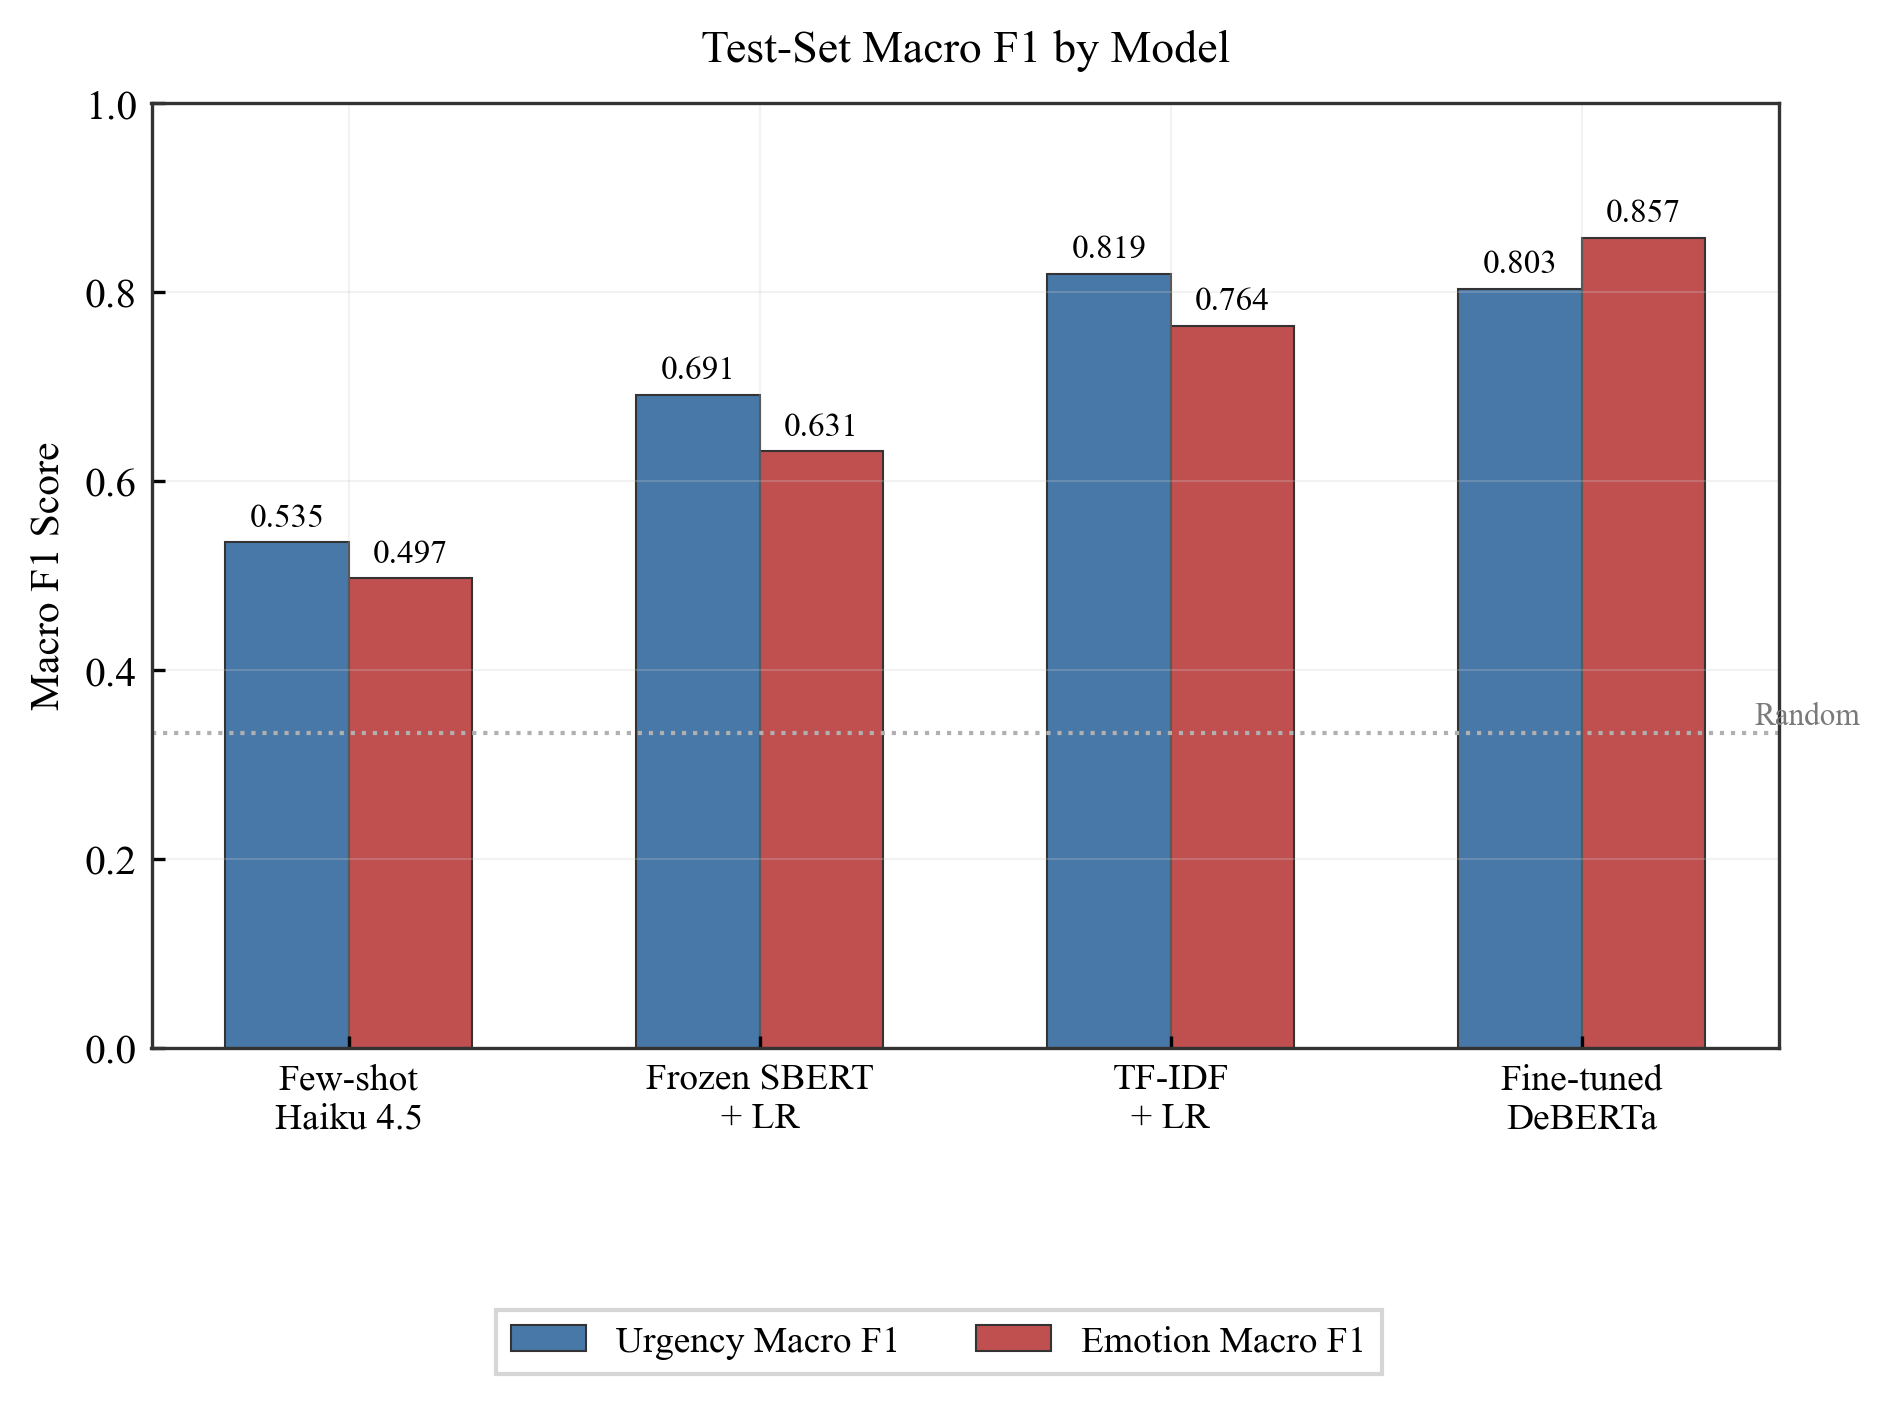
\includegraphics[width=\columnwidth]{figures/fig02_model_comparison.png}
  \caption{Test-set macro F1 by model for urgency and emotion classification.}
  \label{fig:model_comparison}
\end{figure}

The fine-tuned DeBERTa-v3-base achieves the highest combined performance with a mean
macro F1 of 0.830 (urgency 0.803, emotion 0.857), followed by TF-IDF + LR at 0.792,
frozen Sentence-BERT + LR at 0.661, and few-shot Claude Haiku~4.5 at 0.516.
TF-IDF outperforms DeBERTa on urgency by 1.6 percentage points (0.819 vs.\ 0.803),
suggesting that urgency is partly solvable by lexical features alone --- scenario-specific
n-grams like ``outage'' or ``disconnected'' provide strong class signal without
contextual understanding. DeBERTa's advantage concentrates on emotion, where it gains
9.3 percentage points over TF-IDF (0.857 vs.\ 0.764), as emotion classification
requires interpreting tone, register, and pragmatic intent that bag-of-words features
cannot capture.

The frozen SBERT baseline underperforms TF-IDF on both dimensions by over 12 percentage
points, reflecting a domain gap: all-MiniLM-L6-v2 optimises for paraphrase detection,
compressing complaints into a semantic space that discards fine-grained lexical signals.
Few-shot Haiku~4.5 scores lowest, consistent with \citet{roumeliotis2025}, who observe
that general-purpose LLMs struggle with fine-grained ordinal distinctions without
task-specific training, and with \citet{tornberg2024finetuned}, who demonstrate that
fine-tuned smaller models consistently outperform zero-shot generative models on
classification tasks.

\begin{figure}[H]
  \centering
  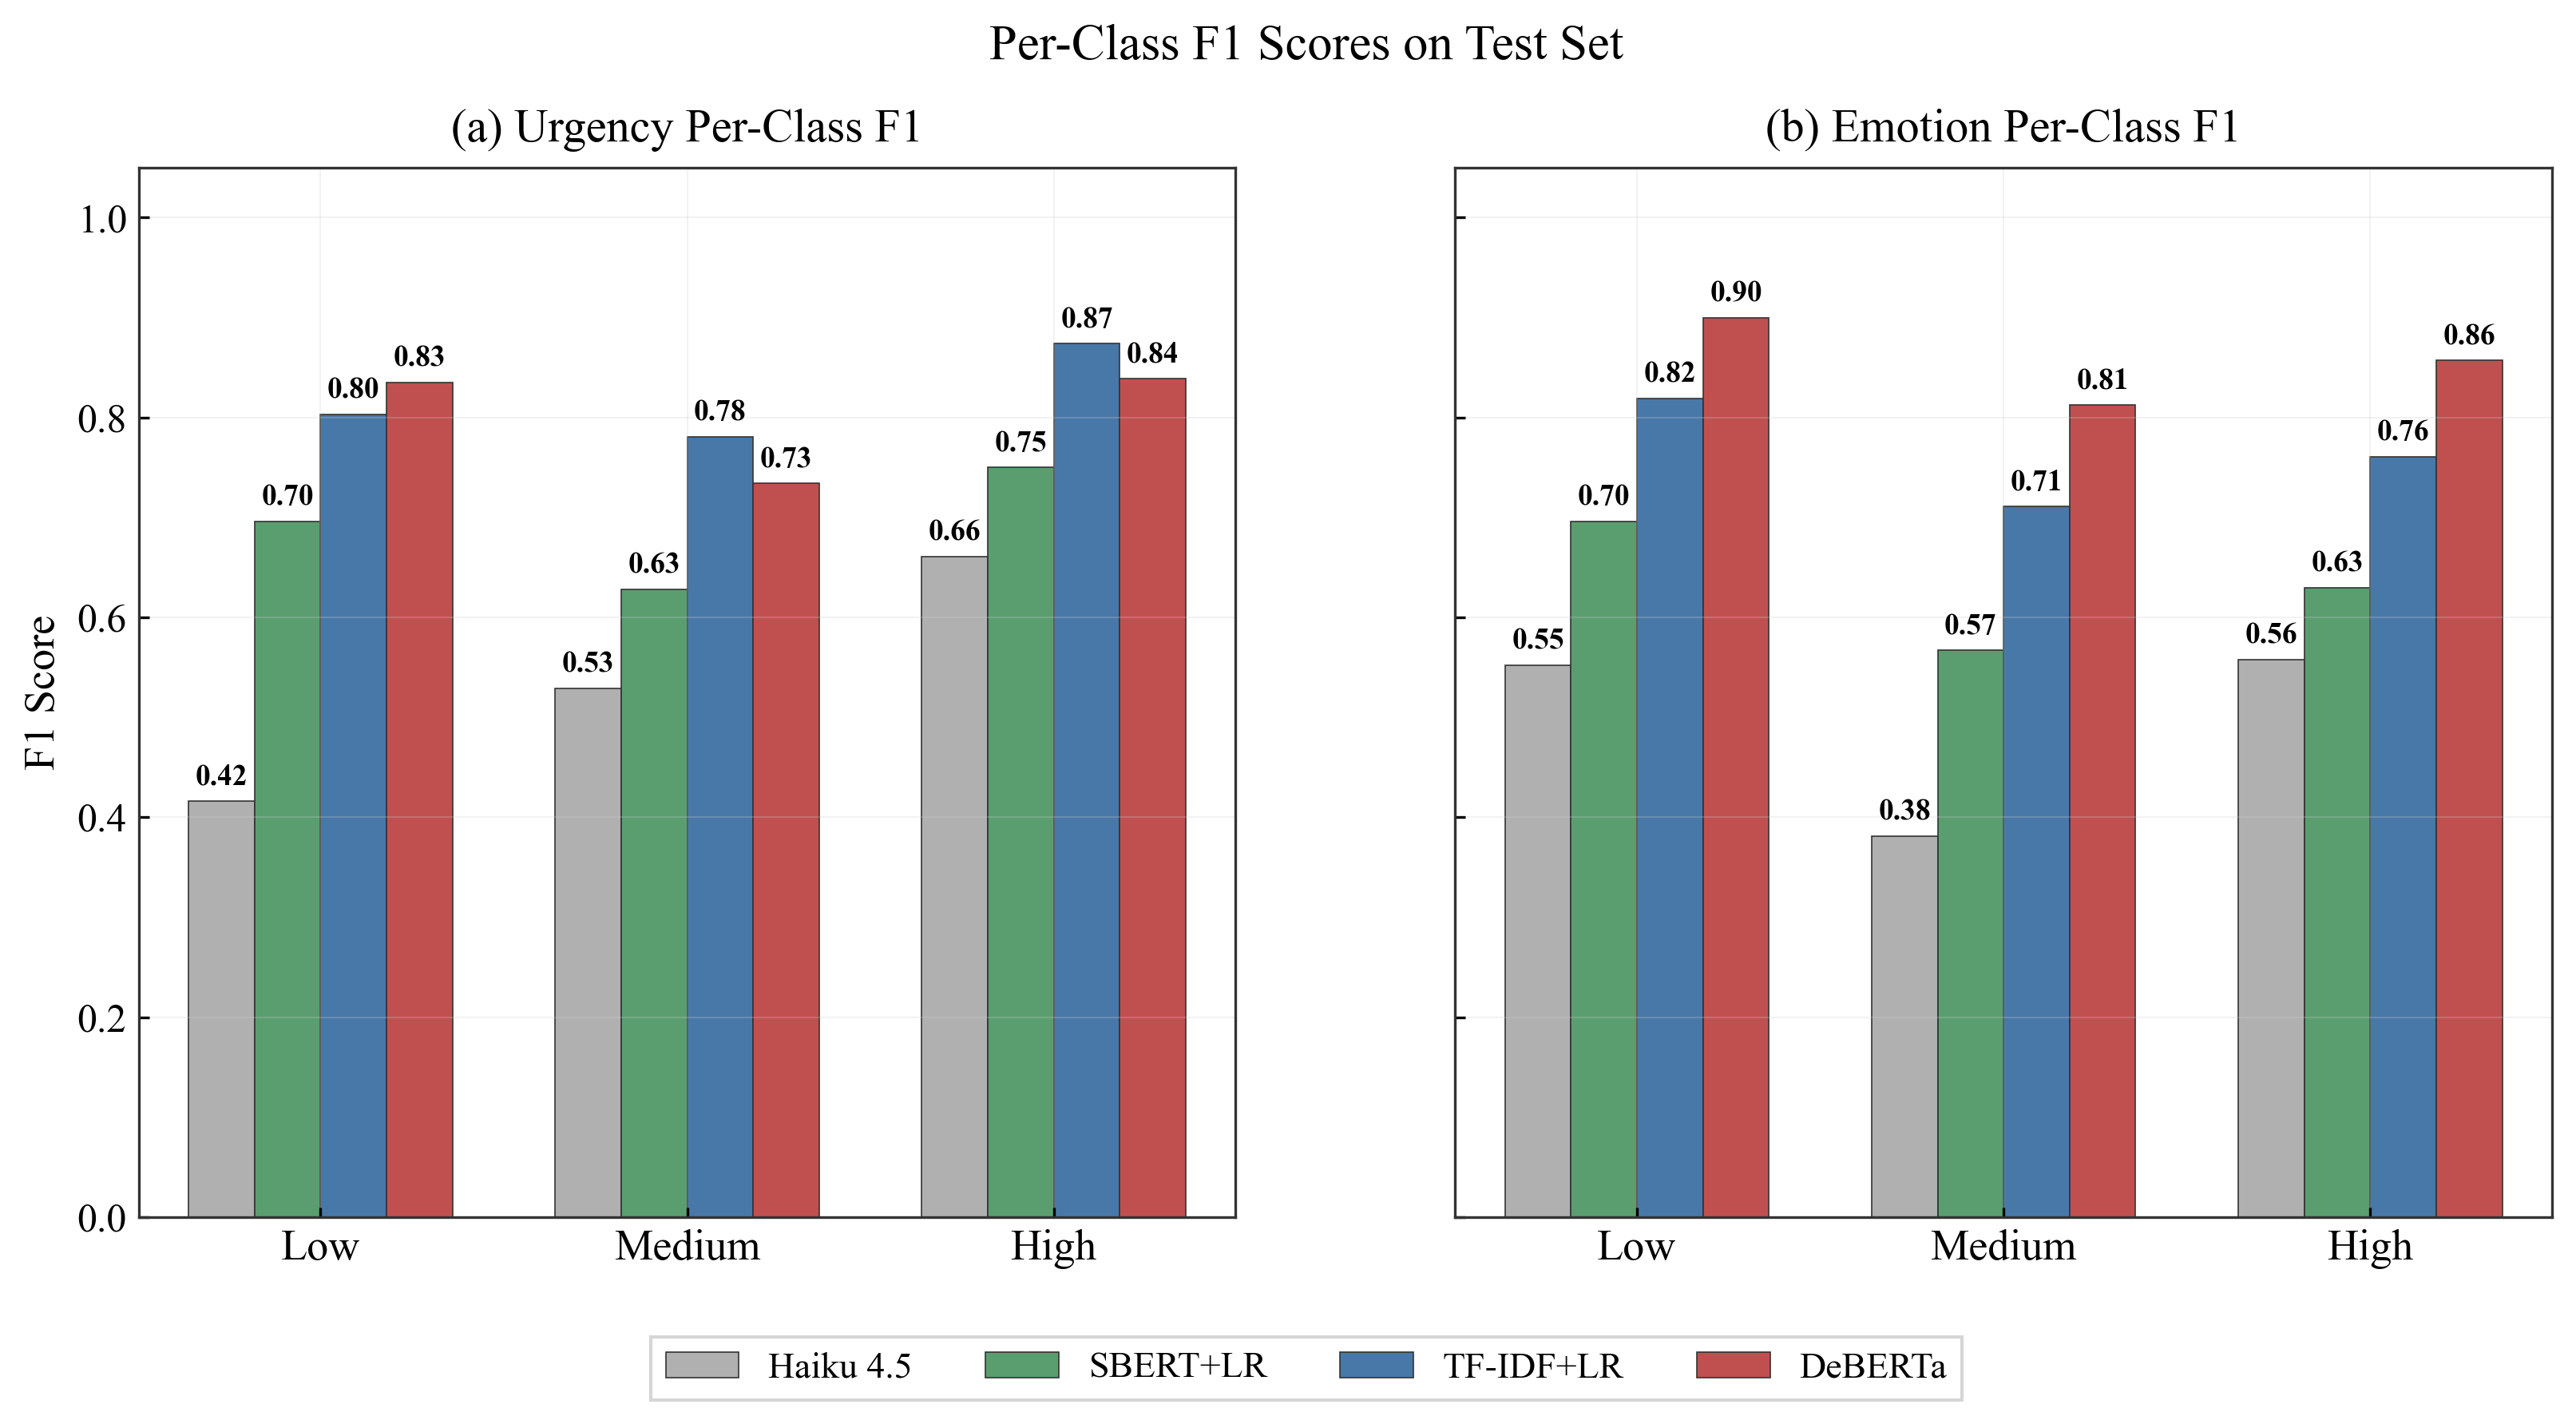
\includegraphics[width=\columnwidth]{figures/fig03_per_class_f1.png}
  \caption{Per-class F1 scores on the test set across models and dimensions.}
  \label{fig:per_class}
\end{figure}

A class-level breakdown of F1 scores across models and dimensions further clarifies
this pattern. Medium is the worst-performing class across every model and both
dimensions. This is consistent with \citet{lu2024mitigating}, who demonstrate that
classifiers, large language models included, systematically concentrate confusion at
middle categories, where decision boundaries between adjacent classes are least
separable. DeBERTa's urgency Medium F1 (0.734) trails Low (0.835) and High (0.839) by
approximately 10 percentage points.
\subsection{Dataset Versioning with DeBERTa-v3}
\label{sec:versioning}

\begin{figure}[H]
  \centering
  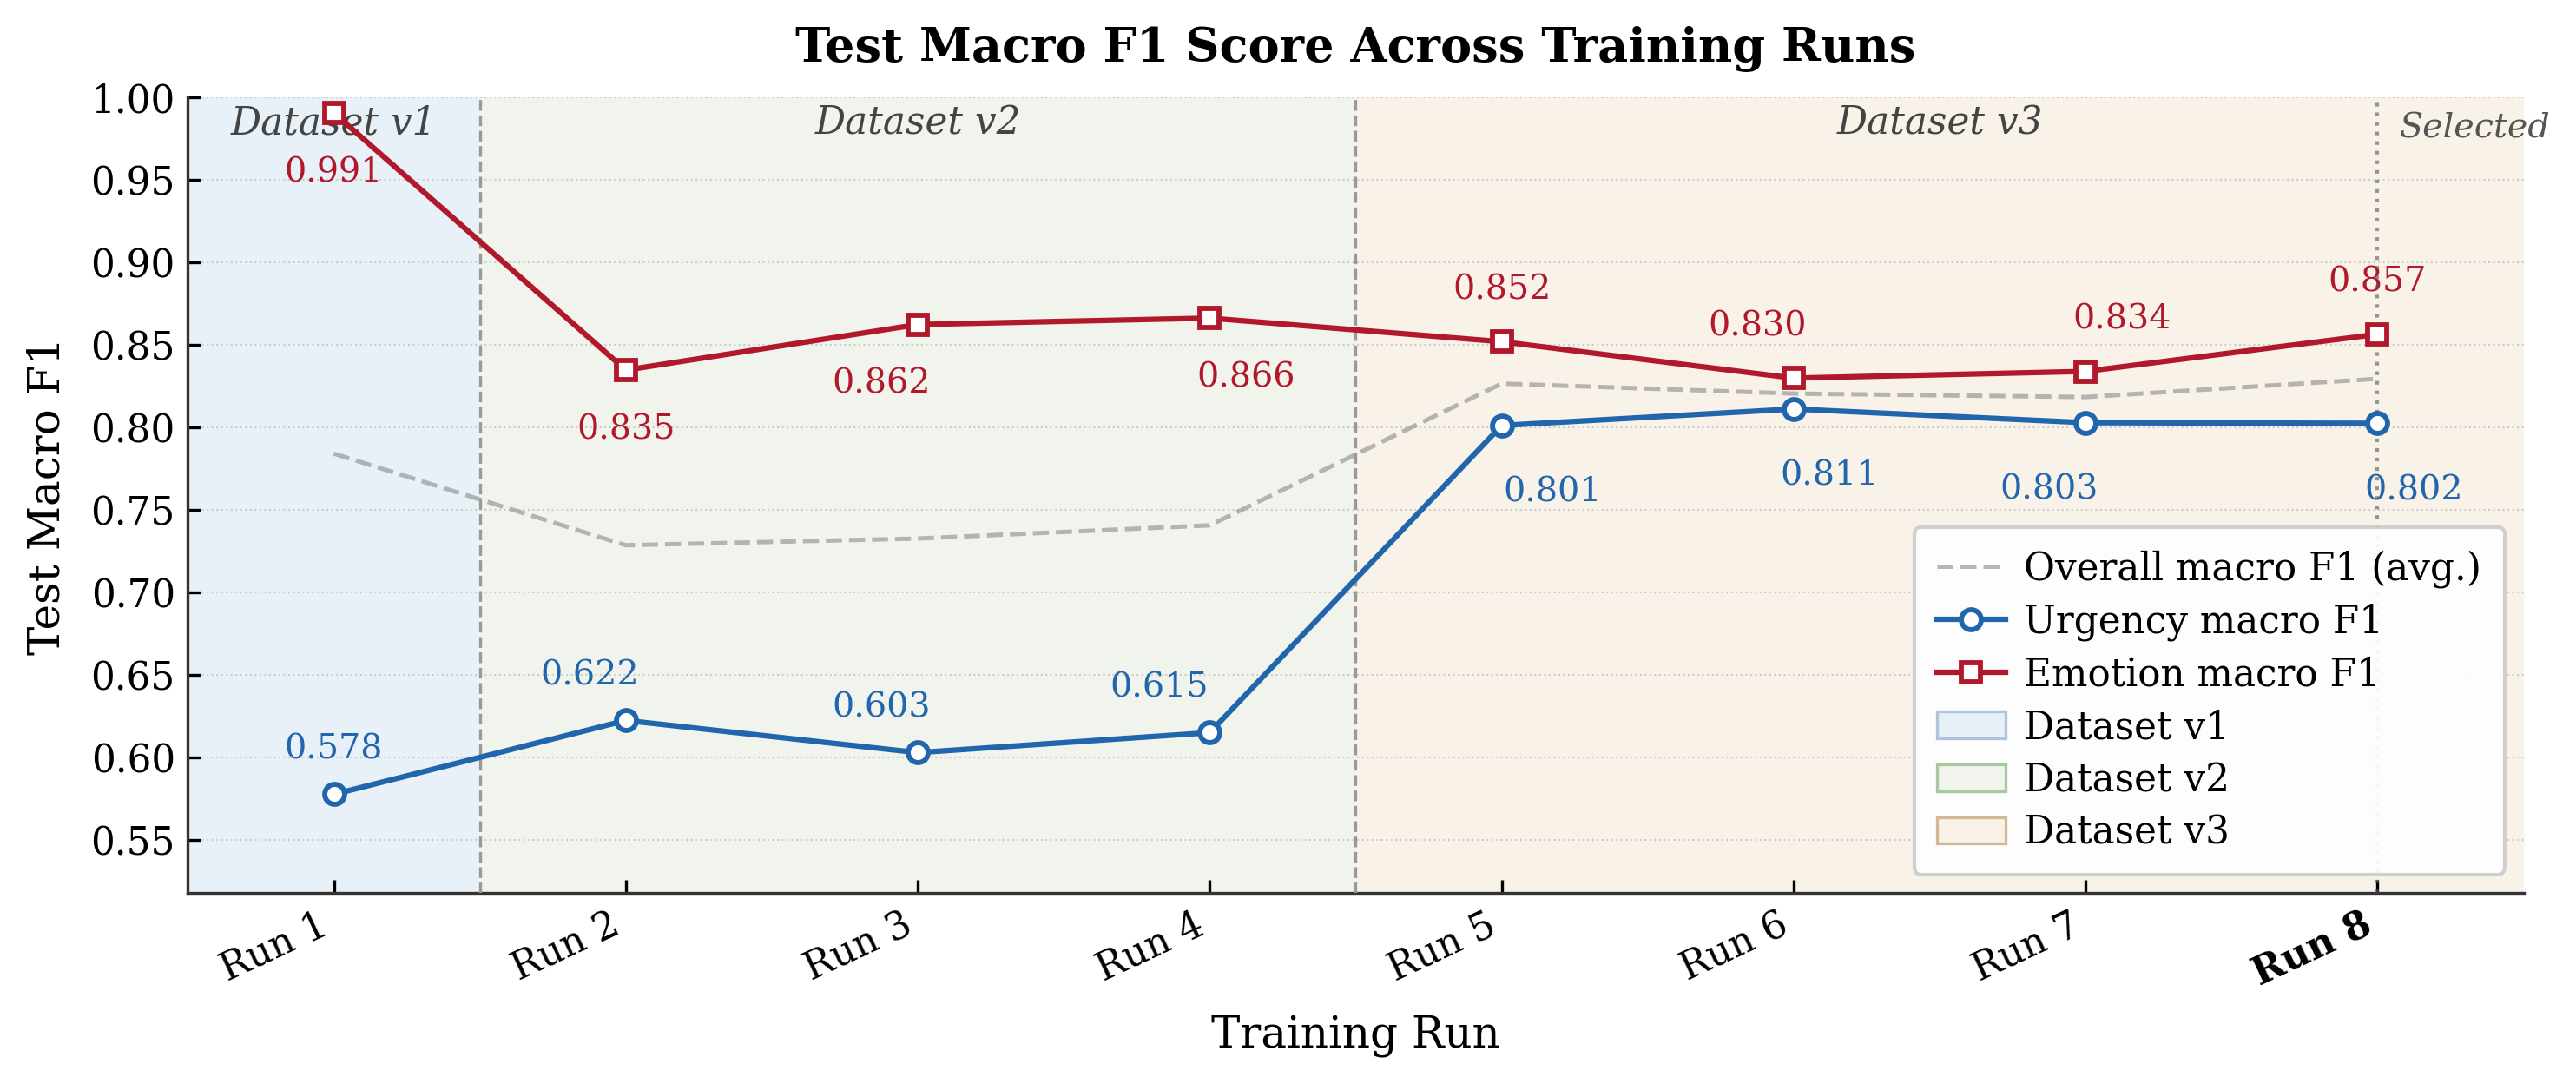
\includegraphics[width=\columnwidth]{figures/fig04_training_runs.png}
  \caption{Test macro F1 score across eight training runs spanning three dataset
  versions, illustrating the impact of data quality on model performance.}
  \label{fig:versioning}
\end{figure}

Figure~\ref{fig:versioning} traces DeBERTa-v3-base test performance across eight
training runs spanning three dataset versions, illustrating how classification quality
evolved as a function of data quality rather than model configuration.

The single run on Dataset v1 produced an emotion macro F1 of 0.991, an implausibly
high result that confirmed the data leakage described in Section~2.3. The model had
effectively learned a vocabulary lookup table rather than any genuine emotional
understanding, rendering the result uninformative as a measure of classification
capability.

Dataset v2 corrected the leakage artefacts, and emotion macro F1 fell to a credible
range of 0.835 to 0.866 across three runs with varying hyperparameters. However,
urgency macro F1 remained invariant across those same runs, spanning only 0.603 to
0.622 regardless of changes to learning rate, class weights, and sequence length. The
narrow range of urgency scores across three independently configured runs is the key
diagnostic: if the ceiling were a modelling problem, hyperparameter changes would have
produced some variation. The fact that they did not pointed unambiguously to a data
quality constraint.

The transition to Dataset v3 produced an immediate and substantial improvement in
urgency macro F1, rising from 0.615 on the final v2 run to 0.801 on the first v3 run,
an increase of 18.6 percentage points. This step change, achieved without any
modification to the model architecture or training configuration, confirms that the v2
urgency ceiling was caused by generation quality rather than model capacity. The finding
aligns with \citet{iskander2024quality}, who empirically demonstrate that models trained
on smaller but higher-quality synthetic datasets consistently outperform those trained on
larger unvalidated sets. Across four runs on Dataset v3, urgency macro F1 remained
stable between 0.801 and 0.811, and emotion macro F1 between 0.830 and 0.857,
indicating that the model had reached a consistent performance level bounded by the v3
dataset. Run~8 was selected as the final model on the basis of achieving the highest
combined macro F1, with an urgency score of 0.802 and an emotion score of 0.857.
Details of each run are presented in Appendix~D.

\subsection{Training Dynamics -- Run 8}

\begin{figure}[H]
  \centering
  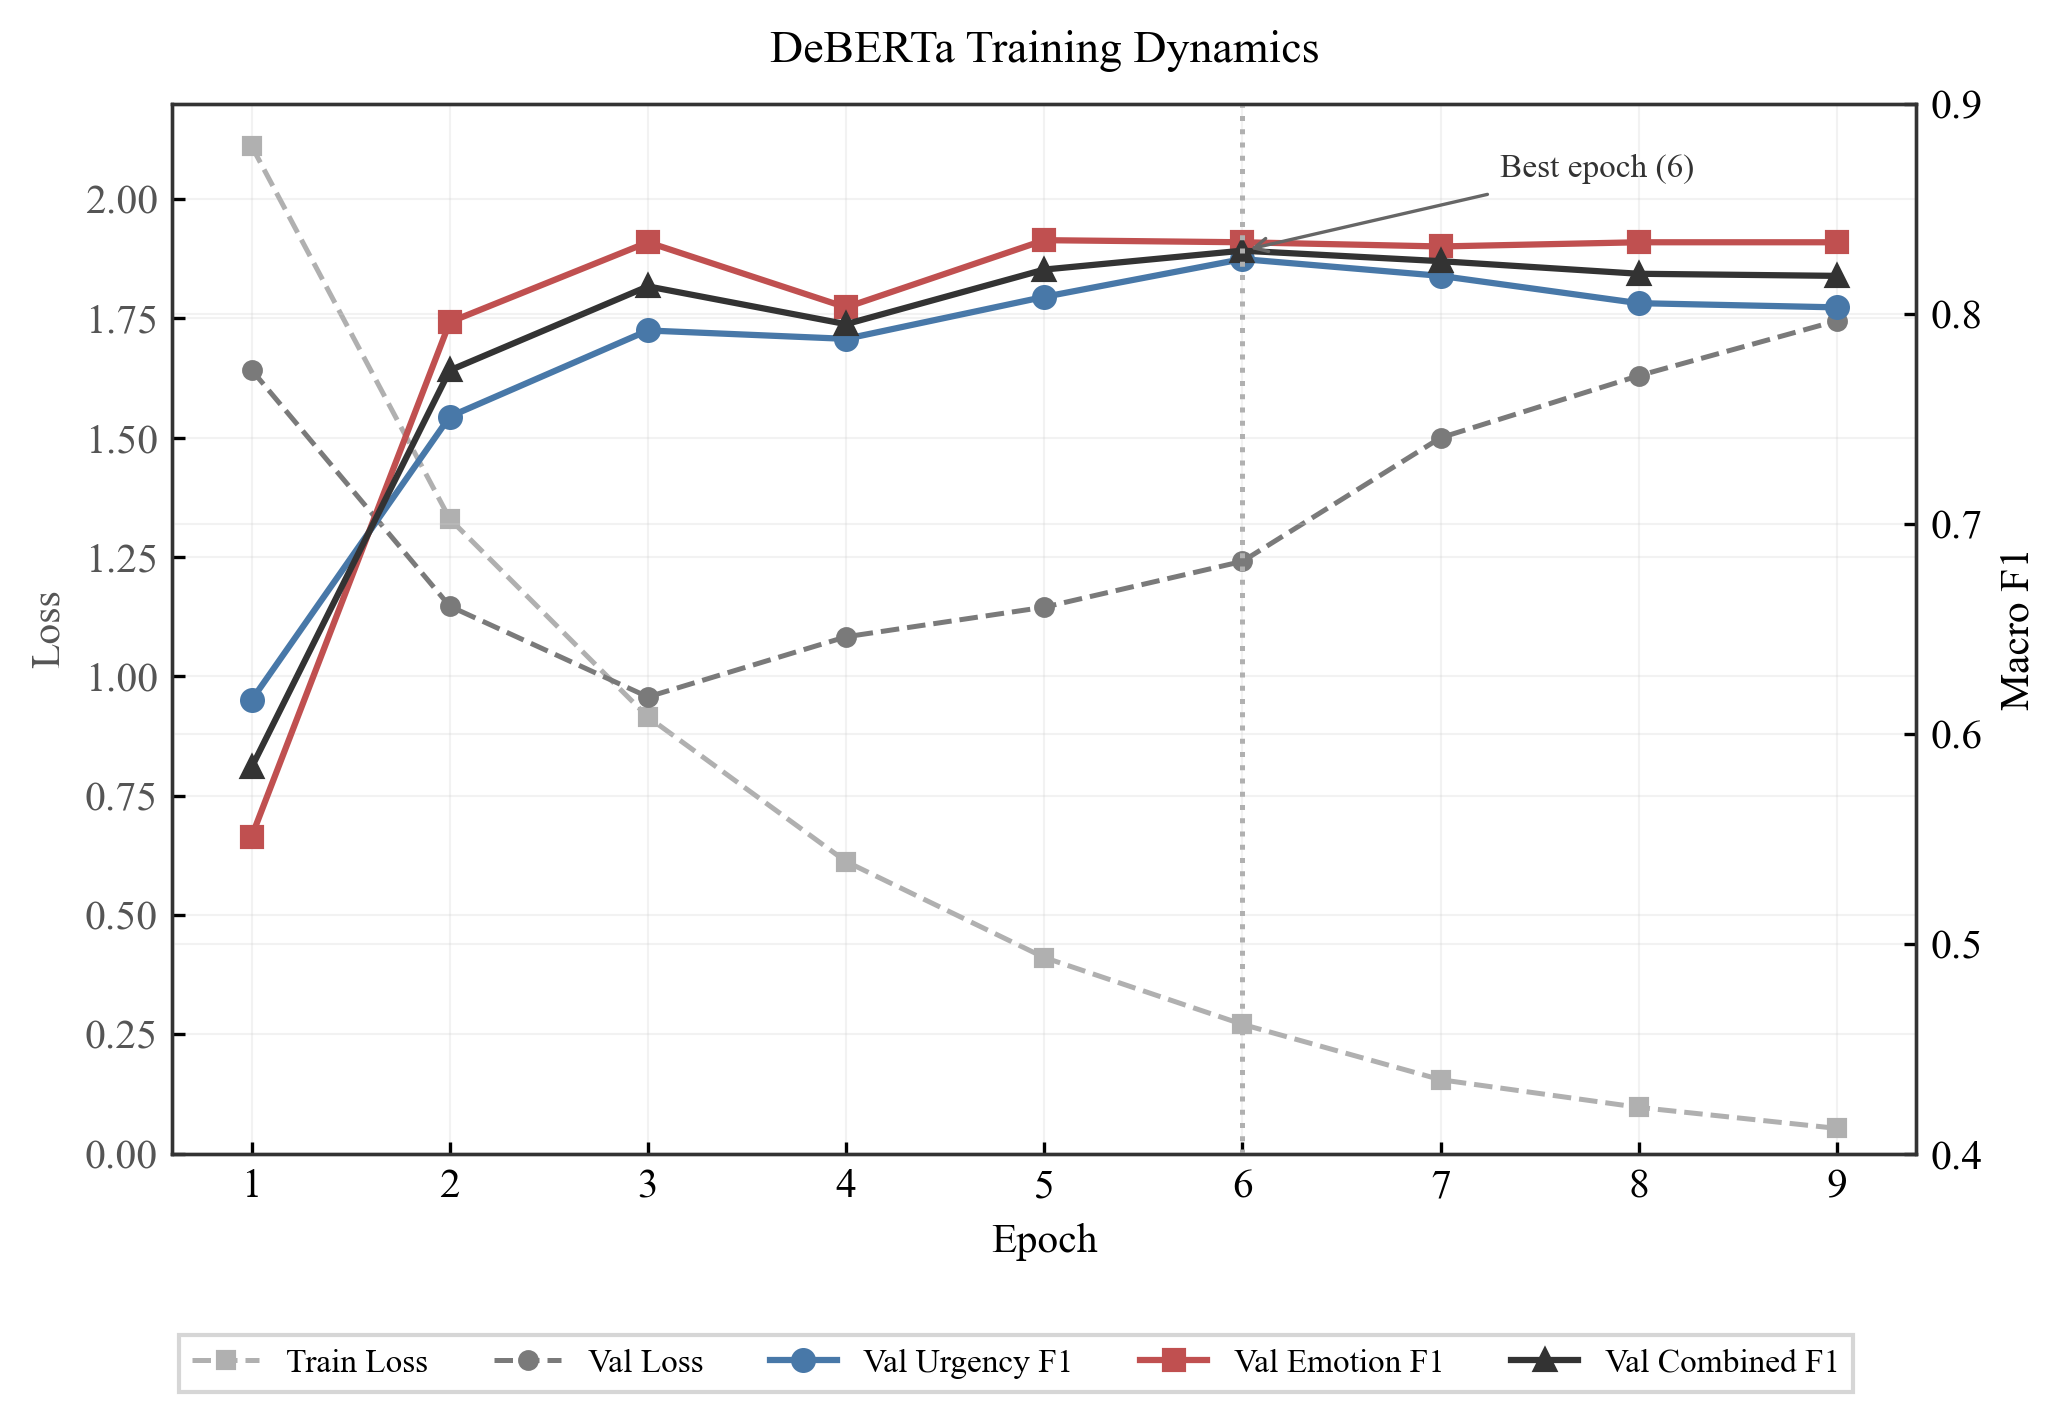
\includegraphics[width=\columnwidth]{figures/fig05_training_dynamics.png}
  \caption{DeBERTa training dynamics for Run~8. Validation loss diverges from training
  loss after epoch~3, yet validation F1 continues improving until epoch~6 where early
  stopping fires.}
  \label{fig:training_dynamics}
\end{figure}

The model was selected at Epoch~6 by early stopping on validation combined F1.
Validation loss diverges from training loss after epoch~3, rising from 0.957 to 1.745,
yet validation F1 continues improving until epoch~6 (combined F1 of 0.830). Had we used
loss-based early stopping, the model would have been selected at epoch~3 (combined F1
of 0.813), forfeiting 1.7 percentage points. The emotion head converges by epoch~3,
while the urgency head continues climbing until epoch~6, consistent with the fact that
urgency requires longer training to synthesise situational details distributed across
complaint texts.

\subsection{Confusion Structure}

\begin{figure}[H]
  \centering
  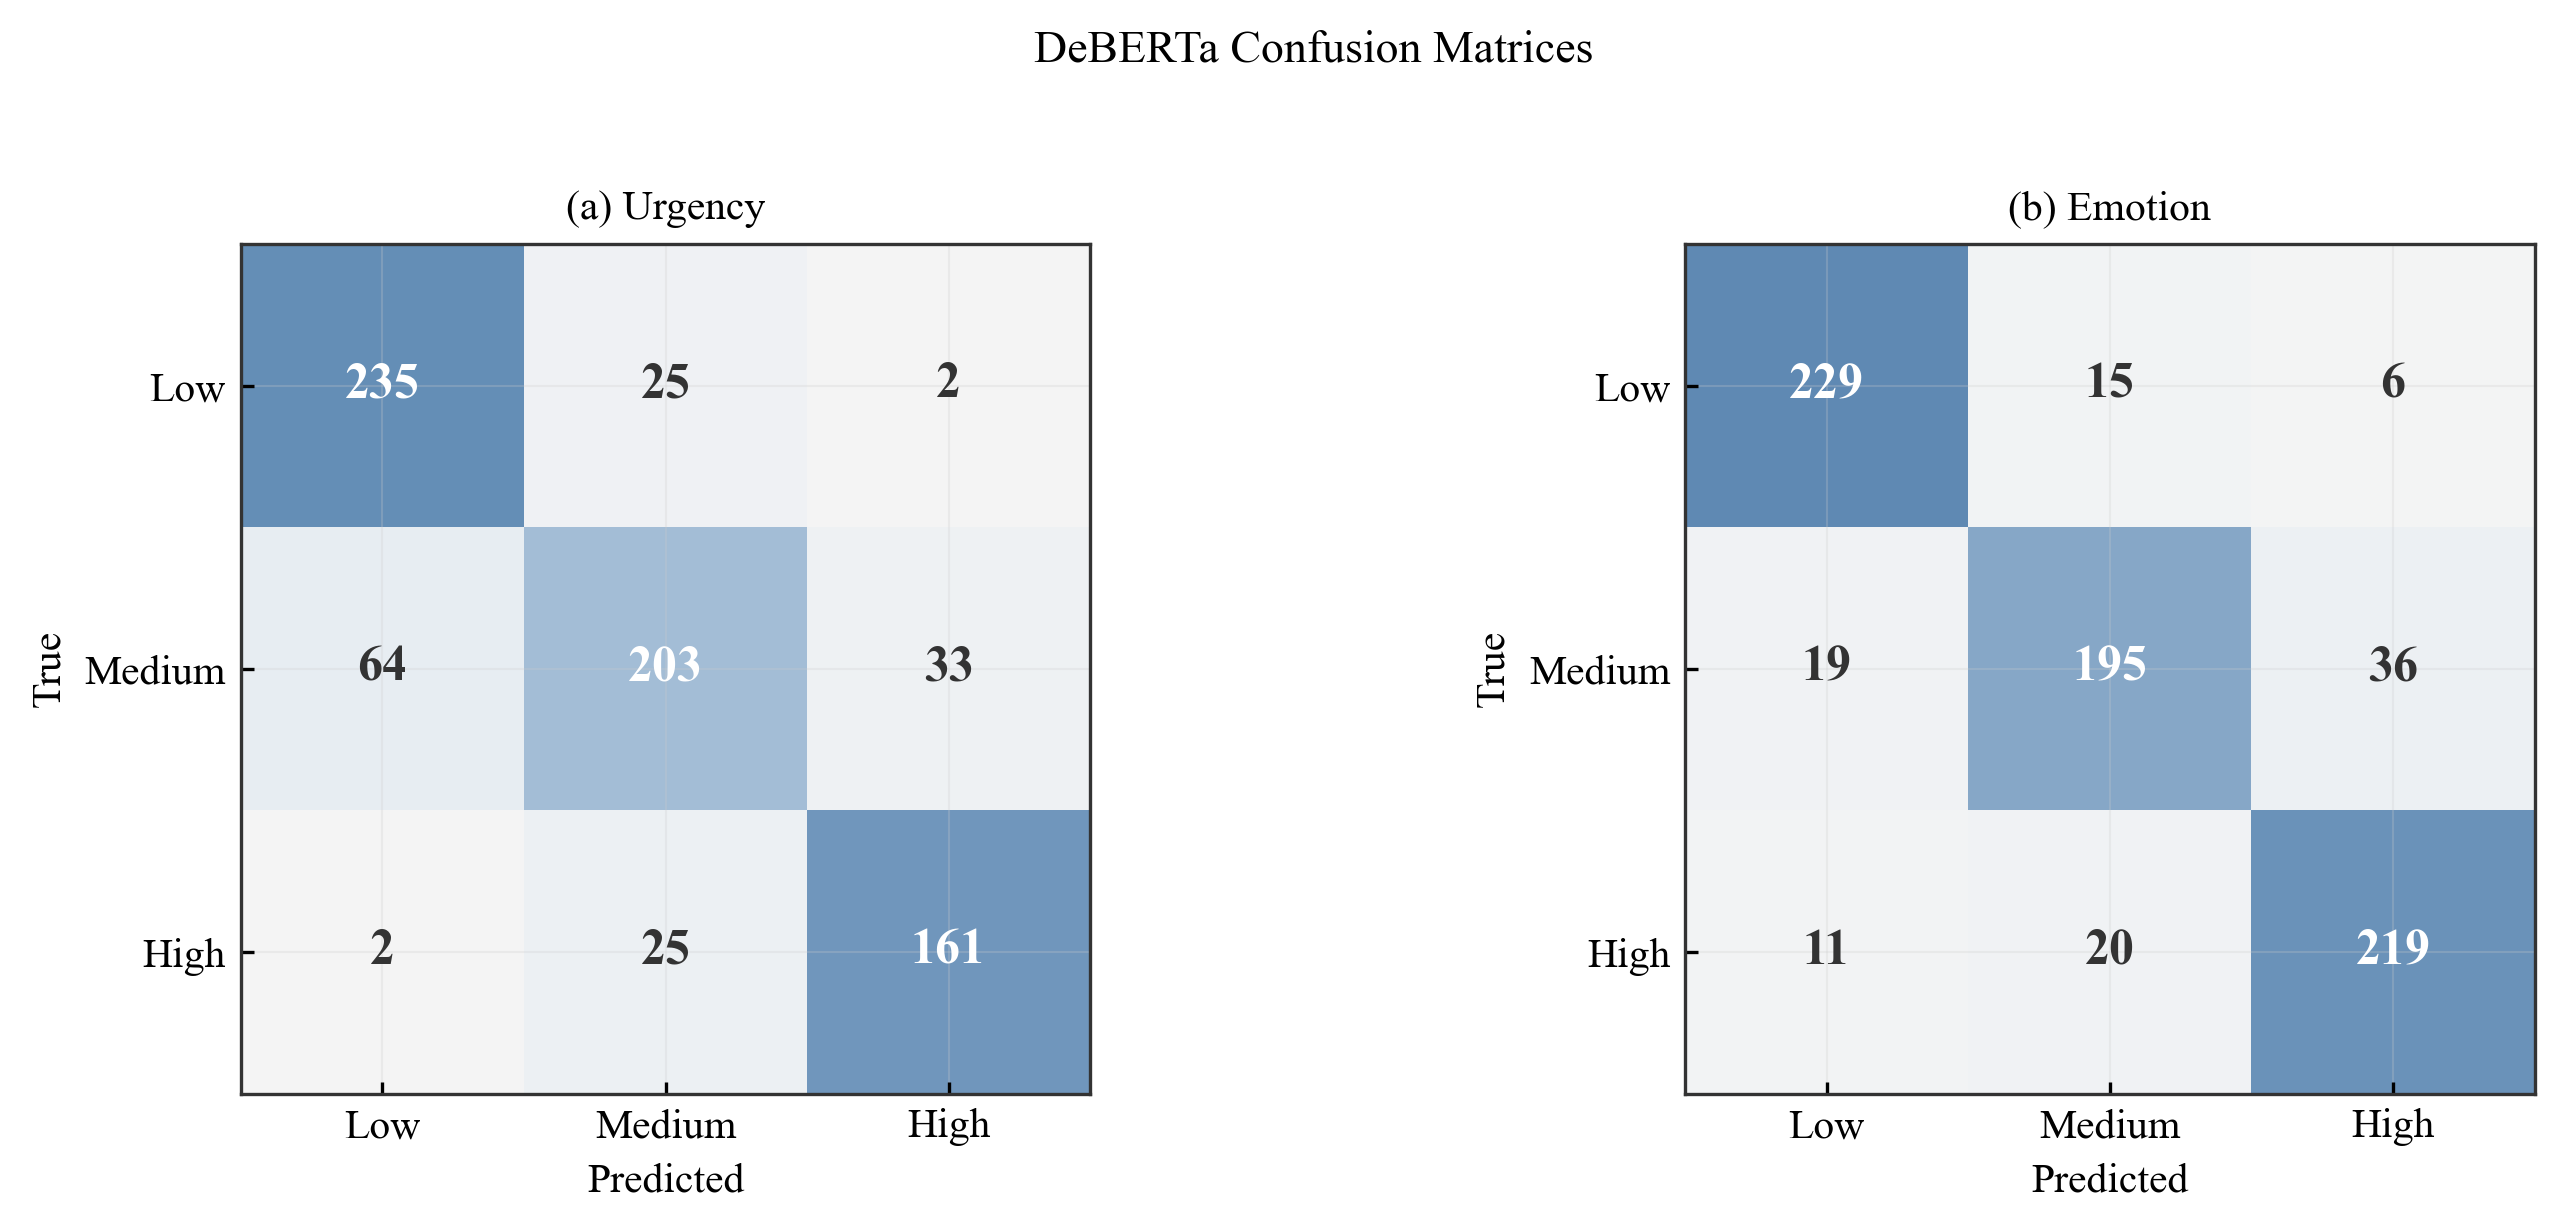
\includegraphics[width=\columnwidth]{figures/fig06_confusion_matrices.png}
  \caption{Confusion matrices for DeBERTa urgency (left) and emotion (right)
  classification on the test set.}
  \label{fig:confusion}
\end{figure}

DeBERTa makes 151 urgency errors (20.1\%) and 107 emotion errors (14.3\%). For urgency,
97.4\% of mistakes are single-step confusions between adjacent classes, which suggests
that the model largely preserves the ordinal structure of the labels. The main
asymmetry, however, is downward error: the most common urgency misclassification is
Medium predicted as Low (64 cases, 42.4\% of urgency errors), and lower-than-true
predictions are more frequent than higher-than-true ones overall. This is also
reflected in the class-wise metrics. Low urgency has high recall (89.7\%) but lower
precision (78.1\%), indicating that the Low class absorbs a substantial number of cases
from higher true classes. Medium shows the weakest recall (67.7\%), largely because
many Medium cases are pushed down into Low, while High remains comparatively stable
with precision of 82.1\% and recall of 85.6\%. Hence, these results suggest a
systematic tendency to under-predict urgency rather than a pattern of random error.
For emotion, the dominant error goes in the opposite direction: Medium is most often
predicted as High (36 cases, 33.6\% of emotion errors), suggesting a mild upward shift
in that head. These error patterns are examined in more detail in the next section.

% ─────────────────────────────────────────────────────────────────────────────
\section{Contrastive Error Analysis}
% ─────────────────────────────────────────────────────────────────────────────

To evaluate the DeBERTa model's dual-head performance beyond standard aggregate metrics,
we implemented a Contrastive Error Analysis pipeline. Rather than looking at aggregate
failure rates, this method systematically matches incorrect predictions with successful
predictions that share the exact same metadata (ground truth label, scenario, and
communication style). These matched Informative Correct Pairs (ICPs) allow us to isolate
specific linguistic, structural, or contextual features, enabling identification of
underlying algorithmic blind spots.

\subsection{Dual-Head Accuracy Comparison}

Evaluating the model reveals a clear discrepancy: it performs significantly better at
classifying Emotion than Urgency. Urgency is inherently more difficult to classify as
it requires deep contextual understanding of socio-economic impact, deadlines, and
technical severity. In practice, the severity of an issue is often defined by
company-internal documents. Emotion, even though nuanced, often has more apparent
vocabulary triggers.

\begin{figure}[H]
  \centering
  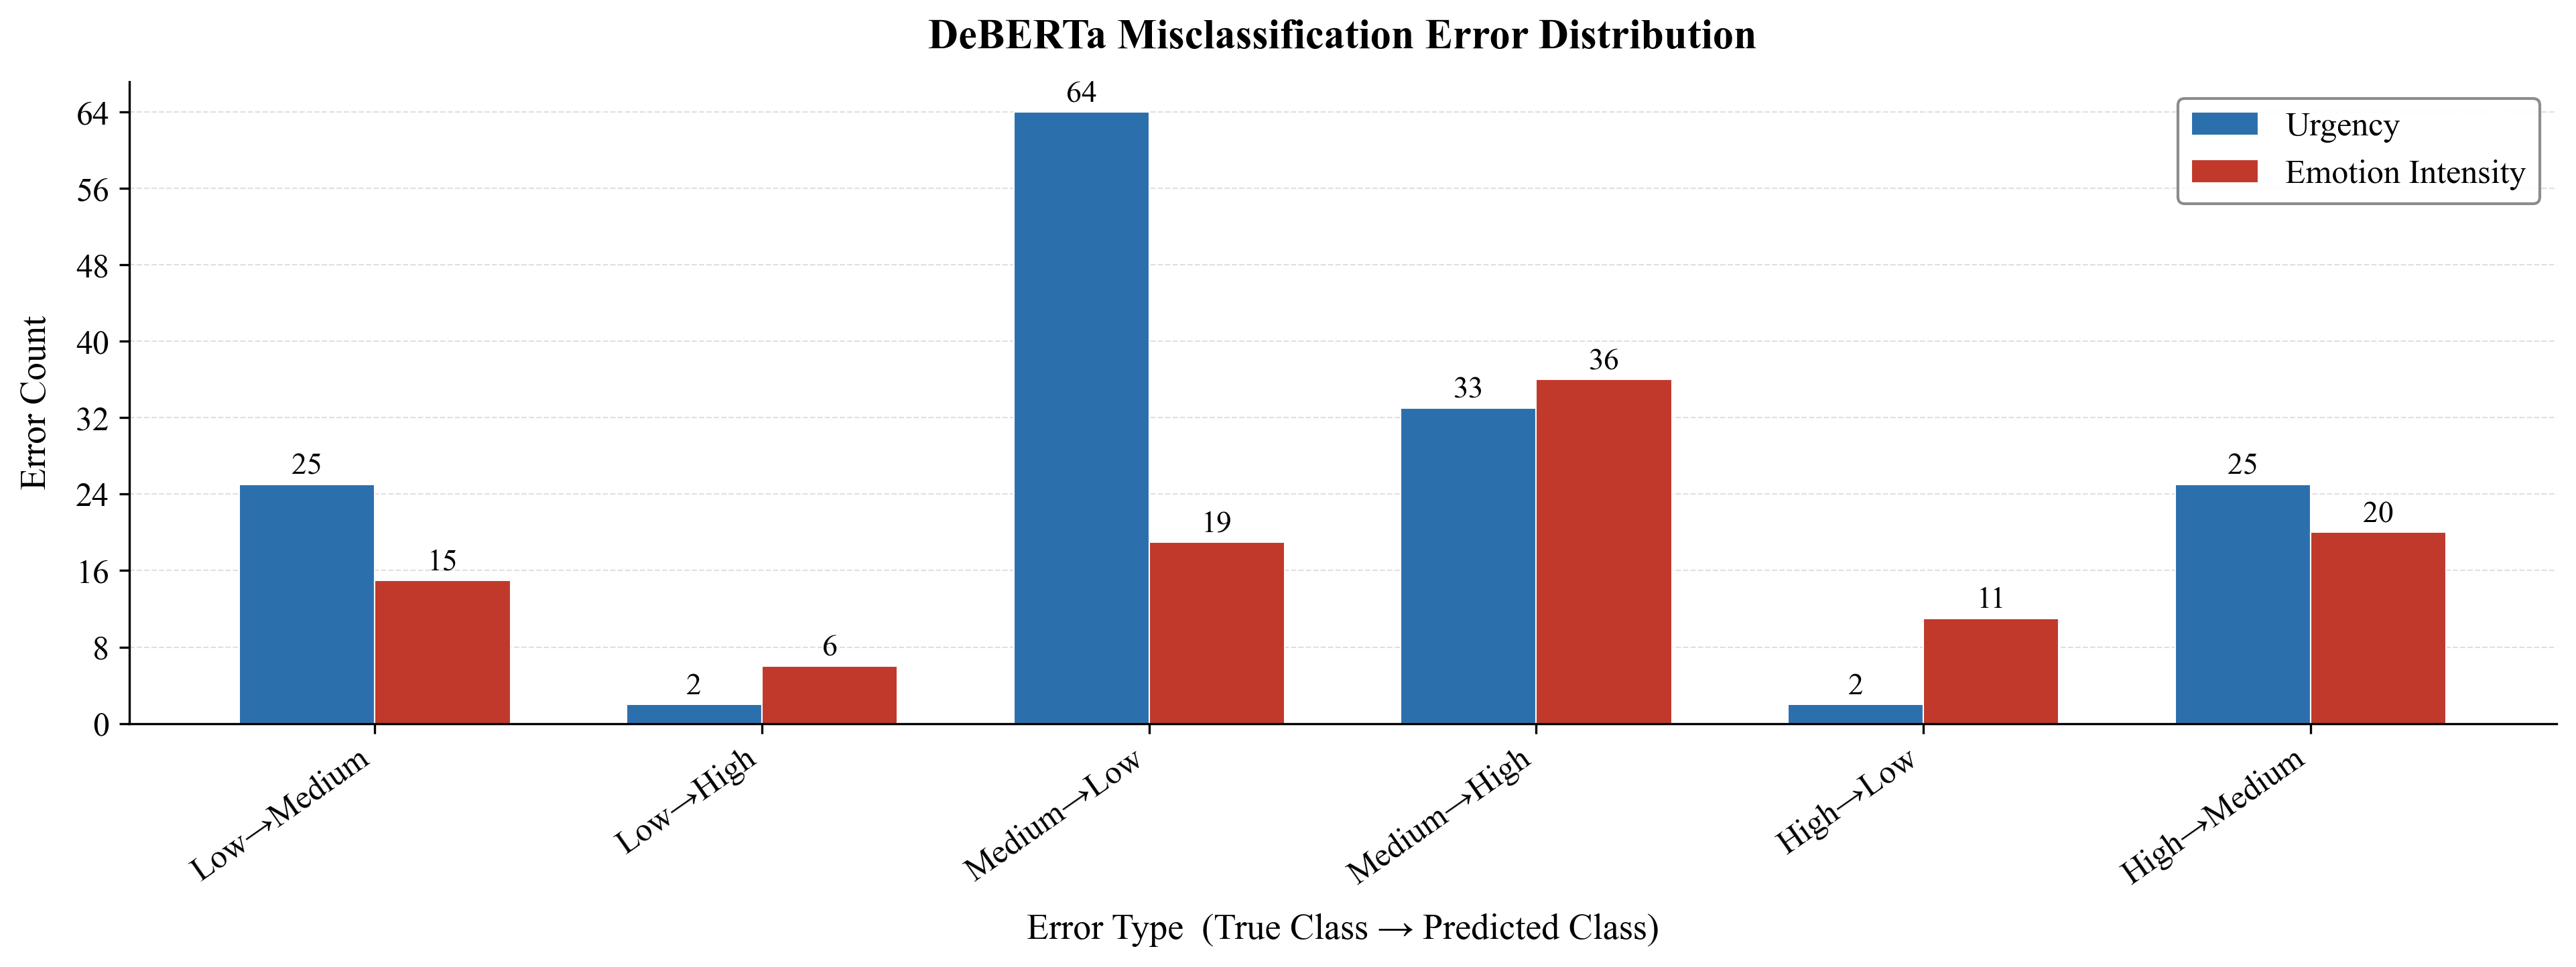
\includegraphics[width=\columnwidth]{figures/fig07_error_distribution.png}
  \caption{DeBERTa misclassification error distribution for urgency (blue) and emotion
  intensity (red), grouped by error type (true class $\to$ predicted class).}
  \label{fig:error_dist}
\end{figure}

\subsection{Urgency Head Analysis}

\begin{table}[H]
  \centering
  \small
  \begin{tabular}{p{3.8cm}p{9cm}}
    \toprule
    \textbf{Blind Spot} & \textbf{Description} \\
    \midrule
    Emotional \& Vulnerability Over-indexing &
      The model misinterprets expressions of emotional distress or personal vulnerability
      as High urgency, while failing to adequately weigh explicit statements of patience
      or willingness to wait. \\
    \addlinespace
    Contextual Misinterpretation of Deadlines &
      The model over-prioritises explicit deadlines or external escalation threats
      (e.g.\ Ombudsman, legal action) without sufficiently contextualising the actual
      impact or immediacy. \\
    \addlinespace
    Failure to Synthesise Problem History &
      The model struggles to weigh the cumulative effect of repeated service failures,
      over-indexing on single recent events instead of persistent crises. \\
    \bottomrule
  \end{tabular}
  \caption{Top 3 urgency head blind spots identified via contrastive error analysis.}
  \label{tab:urgency_blindspots}
\end{table}

\subsection{Emotion Head Analysis}

\begin{table}[H]
  \centering
  \small
  \begin{tabular}{p{3.8cm}p{9cm}}
    \toprule
    \textbf{Blind Spot} & \textbf{Description} \\
    \midrule
    Misinterpreting Cumulative Impact &
      The model struggles to infer emotion from the cumulative weight of repeated issues
      or severe financial strain without explicit high-impact angry keywords. \\
    \addlinespace
    Over-reliance on Overt Aggressive Language &
      The model over-indexes on explicit personal frustration or aggressive `power
      phrases', misclassifying intensity when the tone is strictly formal but legally
      threatening. \\
    \addlinespace
    Under-recognition of Internal Escalation &
      The model fails to identify Medium or High emotional severity in initial contacts
      due to critical system failures without explicit threats. \\
    \bottomrule
  \end{tabular}
  \caption{Top 3 emotion head blind spots identified via contrastive error analysis.}
  \label{tab:emotion_blindspots}
\end{table}

\subsection{Adversarial Stress Testing}

To validate the blind spots identified through contrastive analysis, we constructed 10
targeted adversarial cases, each designed to isolate a specific failure mode. These
cases serve as qualitative illustrations, each either confirming or challenging the
diagnosed blind spot. Notably, the four cases that produced incorrect predictions
mapped precisely onto Blind Spots 1, 2, and 3, providing targeted evidence that the
contrastive analysis correctly identified the model's failure modes.

The adversarial suite was also run against the model trained on Dataset v2 as a
comparative baseline. That earlier model passed only 3 out of 10 cases, whereas the
final v3 model passed 6 out of 10, a meaningful improvement consistent with the broader
performance gains reported in Section~4.2 and attributable to the higher label fidelity
of the v3 dataset.

For example, the adversarial test `Passive-Aggressive Legal Threat' (True Emotion:
High, Predicted: Low) failed exactly as predicted by Emotion Blind Spot 2, as it lacked
explicit angry words but carried extreme threat. Similarly, `Sarcastic Praise' failed
because the model misinterpreted cumulative impact, consistent with Emotion Blind
Spot 1, when the genuine frustration was masked by outwardly positive language.
These complementary results confirm the robustness of our passive error analysis. While
10 adversarial cases are insufficient for quantitative claims about model robustness,
the value of this analysis lies in the specificity of the failures, as each incorrect
prediction corresponded to a previously identified blind spot, suggesting the
contrastive analysis has diagnostic validity.

% ─────────────────────────────────────────────────────────────────────────────
\section{Limitations}
% ─────────────────────────────────────────────────────────────────────────────

The model is trained exclusively on machine-generated text, meaning it learns linguistic
patterns, vocabulary, and rhetorical structures characteristic of large language models
rather than genuine human writing. Real-world complaints tend to be considerably more
chaotic, incorporating severe spelling errors, SMS abbreviations, and
stream-of-consciousness formatting that the synthetic corpus does not capture. Although
adversarial testing partially mitigates this, it cannot fully replicate the noise
present in live production environments.

The dataset is constructed around a fixed set of scenarios, writing styles, and customer
profiles, with strict logical rules governing label assignments, for instance, a scenario
classified as ``Complete Service Outage'' cannot be assigned Low urgency. While this
design ensures internal consistency, real customers routinely produce contradictory
complaints that violate such boundaries, and the full range of real-world
telecommunications situations extends considerably beyond the controlled grid used here.

The model is evaluated exclusively on a held-out partition of the same synthetic dataset
used for training, meaning that reported performance reflects generalisation within a
controlled generative distribution rather than to real-world data. Without validation on
genuine telecoms complaints, it remains uncertain whether the classification boundaries
learned from synthetic text transfer to the broader linguistic variation present in live
production environments. This represents the most consequential constraint on the
external validity of the reported results.

% ─────────────────────────────────────────────────────────────────────────────
\section{Conclusion}
% ─────────────────────────────────────────────────────────────────────────────

This paper examined whether urgency and emotional intensity, two dimensions often
conflated in automated complaint triage, can be separated through deliberate dataset
design and task-specific modelling. The results suggest they can be decoupled to a
practically useful extent within a controlled synthetic setting, while also revealing
where this separation remains difficult.

Among the four evaluated models, the fine-tuned DeBERTa-v3-base achieved the strongest
balanced performance, reaching a combined macro F1 of 0.830 (urgency 0.803, emotion
0.857). TF-IDF marginally outperformed DeBERTa on urgency alone, indicating that part
of the urgency signal is recoverable from lexical cues and scenario-specific wording,
whereas DeBERTa's clear advantage on emotion suggests that emotional intensity depends
more heavily on contextual and pragmatic interpretation. The poor performance of frozen
Sentence-BERT further indicates that general-purpose semantic embeddings are
insufficient for this task.

The dataset versioning process was central to the final outcome. The 18.6
percentage-point improvement in urgency macro F1 between Dataset v2 and v3 strongly
suggests that generation quality was a major constraint, reinforcing the principle that
in synthetic pipelines, improving the training signal can matter at least as much as
model selection \citep{iskander2024quality}.

The contrastive error analysis identified recurring blind spots in both heads, and
adversarial testing was consistent with the diagnosed blind spots, providing preliminary
support for the ICP-based methodology. The dual-head framework provides the technical
foundation for an automated complaint prioritisation system: by separating operational
urgency from emotional intensity, telecom firms could improve routing, prioritisation,
and customer handling, leading to faster escalation of critical cases, more appropriate
agent responses, and more consistent large-scale complaint management. In the UK telecoms
context, this carries direct regulatory relevance, as Ofcom requires prioritised handling
of vulnerable customer complaints, a requirement the emotion head can help operationalise
at scale.

Validation on real telecom data is the most important next step, alongside a data
augmentation strategy that injects adversarial edge cases targeting the identified blind
spots, such as formal legal threats conveying high emotion, to recalibrate the model's
decision boundaries.

% ─────────────────────────────────────────────────────────────────────────────
\newpage
\bibliography{references}
% ─────────────────────────────────────────────────────────────────────────────

\newpage
\appendix
\section*{Appendices}

% ── Code and Data Availability ───────────────────────────────────────────────

\section{Code and Data Availability}

All code and data for this project are publicly available at:

\begin{center}
  \url{https://github.com/tao-yuansheng/nlp_urgency_ranking}
\end{center}

The repository includes: the synthetic dataset generation scripts and all three
dataset versions (v1--v3); baseline model implementations (TF-IDF, Sentence-BERT,
Claude Haiku); the DeBERTa-v3-base multi-task fine-tuning pipeline with all eight
training run configurations; the contrastive error analysis and adversarial stress
testing scripts; and the figure generation code used in this report.

% ── AI Tool Acknowledgment ───────────────────────────────────────────────────

\section{Generative AI Tool Acknowledgment}

This project used generative AI tools in an assistive capacity, consistent with
the MSIN0221 ``Assistive'' AI category. Specifically:

\begin{itemize}
  \item \textbf{OpenAI GPT-5-mini} was used to generate the synthetic complaint
    dataset (Sections 2.2--2.3). All generated complaints were reviewed for
    label-to-text fidelity, and dataset quality was validated iteratively through
    model performance diagnostics.
  \item \textbf{Anthropic Claude Haiku~4.5} was used as a few-shot classification
    baseline (Section 3.2). Its outputs were evaluated solely as model predictions
    on the held-out test set.
  \item \textbf{Claude Code (Anthropic)} was used in an assistive role to support
    code development, debugging, and report formatting. All analytical decisions,
    interpretations, and written content represent the authors' own work.
\end{itemize}

% ── Tables ───────────────────────────────────────────────────────────────────

\section{Adversarial Stress Test Outcomes}

Results of the 10-item adversarial evaluation used to probe decoupled urgency--emotion
reasoning under sarcasm, legal threats, and emotional masking.

\begin{table}[H]
  \centering
  \small
  \resizebox{\textwidth}{!}{%
  \begin{tabular}{clcccp{6cm}}
    \toprule
    \textbf{ID} & \textbf{Case} & \textbf{Expected U/E} & \textbf{Predicted U/E} & \textbf{Result} & \textbf{Why Difficult} \\
    \midrule
    01 & Sarcastic Praise                & Med / High  & High / Low  & FAIL & Glowing words mask intense frustration \\
    02 & Polite Catastrophe              & High / Low  & High / Low  & PASS & Full outage described with total calm \\
    03 & Aggressive Triviality           & Low / High  & Low / High  & PASS & Maximum fury over a cosmetic change \\
    04 & Passive-Aggressive Legal Threat & High / High & Low / Low   & FAIL & Cold legal language, no exclamation marks \\
    05 & Rambling Confusion              & Low / Low   & Low / Low   & PASS & Long message; mild self-billing confusion \\
    06 & Urgent but Cheerful             & High / Low  & High / Low  & PASS & Complete call failure reported with enthusiasm \\
    07 & Sincere Heartbreak              & Low / High  & Low / High  & PASS & Deep sadness over a minor plan change \\
    08 & Pure Machine Logic              & High / Low  & High / Low  & PASS & Network jargon with zero emotional language \\
    09 & Ambiguous Broken                & Med / Med   & Low / Low   & FAIL & Mild recurring issue, hint of exasperation \\
    10 & Overreaction to a Fix           & Low / High  & Med / Med   & FAIL & Issue resolved; sarcasm signals residual anger \\
    \bottomrule
  \end{tabular}}
  \caption{Adversarial stress test outcomes. U = Urgency, E = Emotion.}
  \label{tab:adversarial}
\end{table}

\section{Training Run Hyperparameters}

Summary of all DeBERTa training runs and the hyperparameter or dataset changes introduced
across iterations.

\begin{table}[H]
  \centering
  \small
  \resizebox{\textwidth}{!}{%
  \begin{tabular}{clcccp{6cm}}
    \toprule
    \textbf{Run} & \textbf{Dataset} & \textbf{Max Len} & \textbf{LR Setup} & \textbf{Max Epochs} & \textbf{Key Change} \\
    \midrule
    1 & v1 & 128 & $2{\times}10^{-5}$                          & 5  & Baseline. Unified LR, FP16, no class weights \\
    2 & v2 & 128 & $2{\times}10^{-5}$                          & 5  & Dataset updated to v2; all settings identical \\
    3 & v2 & 192 & $2{\times}10^{-5}$                          & 10 & Max length 128$\to$192; epochs extended to 10 \\
    4 & v2 & 192 & $1{\times}10^{-5}$                          & 10 & Unified LR halved \\
    5 & v3 & 192 & $2{\times}10^{-5}$                          & 10 & Dataset updated to v3; LR restored \\
    6 & v3 & 192 & $1{\times}10^{-5}$ / $5{\times}10^{-5}$    & 10 & Split LR: lower for encoder, higher for heads \\
    7 & v3 & 192 & $1{\times}10^{-5}$ / $2{\times}10^{-5}$    & 15 & Head LR reduced; weight decay 0.05 added \\
    8 & v3 & 192 & $2{\times}10^{-5}$                          & 10 & Early stopping on combined macro F1 (\textbf{selected}) \\
    \bottomrule
  \end{tabular}}
  \caption{DeBERTa training run hyperparameters across all dataset versions.}
  \label{tab:runs}
\end{table}

% ── Figures ──────────────────────────────────────────────────────────────────

\section{Scenario-Urgency Affinity Matrix}

\begin{figure}[H]
  \centering
  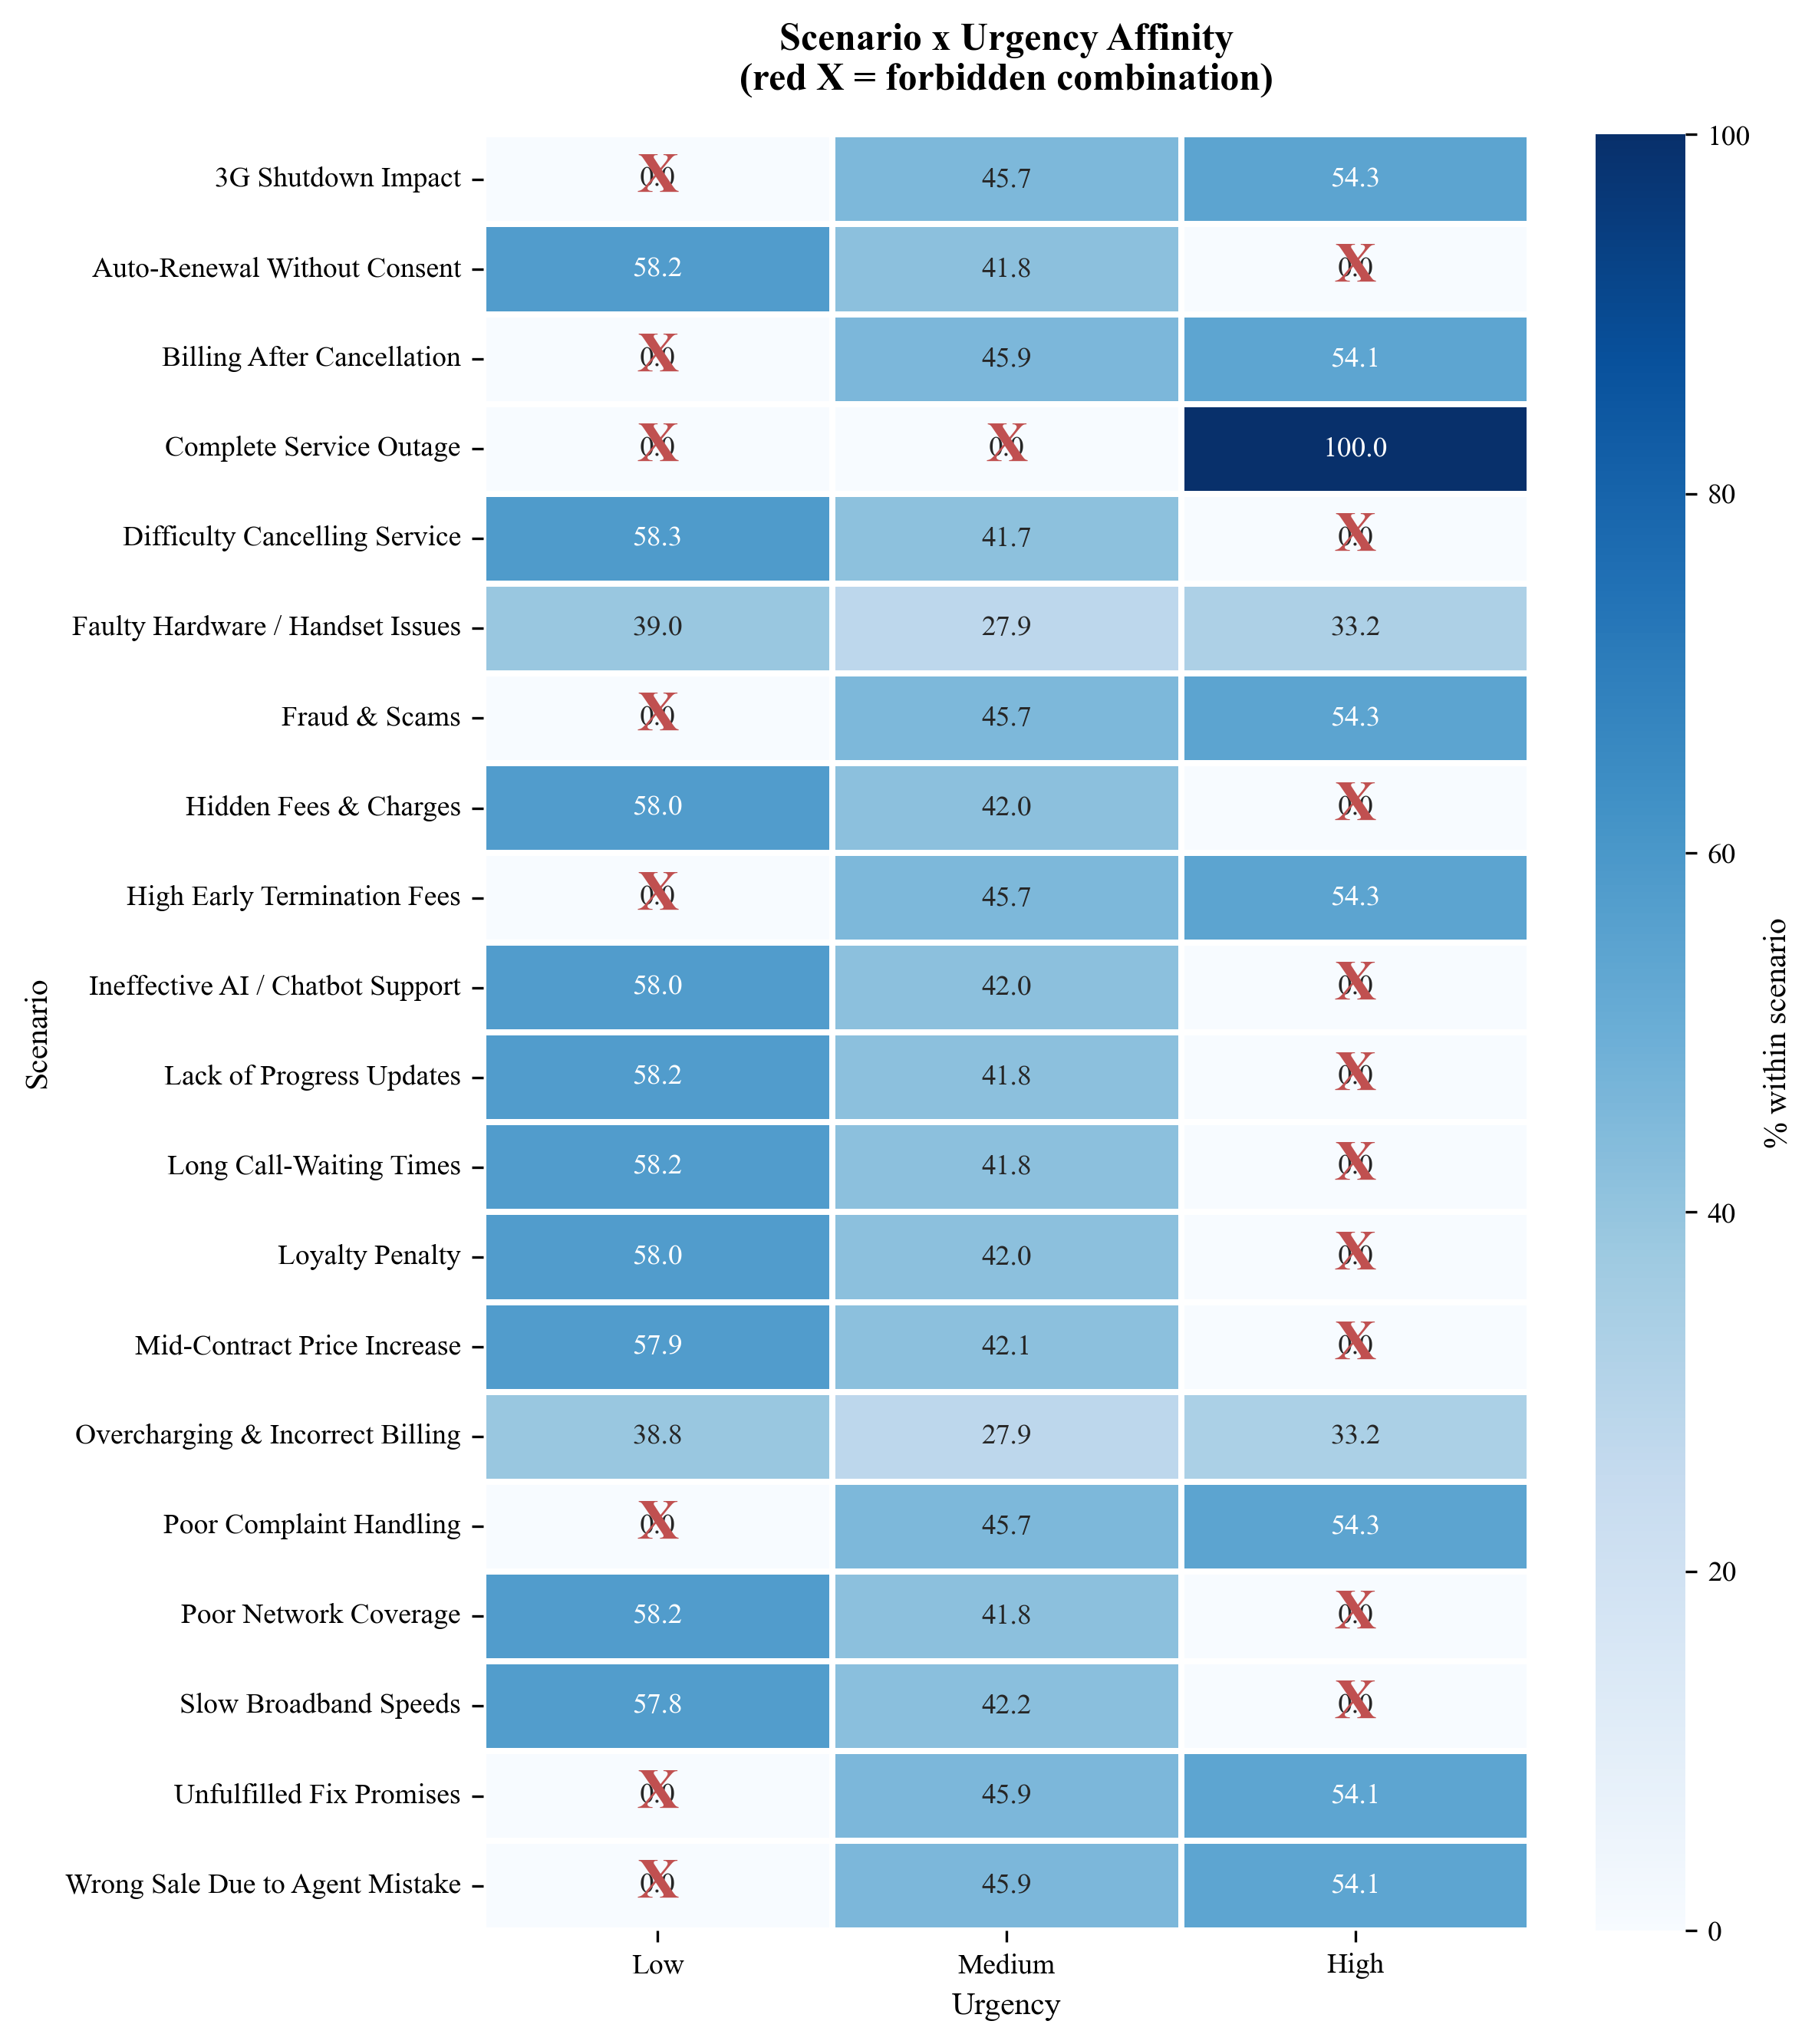
\includegraphics[width=\textwidth]{figures/fig08_scenario_affinity.png}
  \caption{Scenario-urgency affinity matrix showing which UK telecoms complaint
  scenarios were permitted at Low, Medium, and High urgency during synthetic dataset
  construction.}
  \label{fig:affinity}
\end{figure}

\section{Metadata Coverage}

\begin{figure}[H]
  \centering
  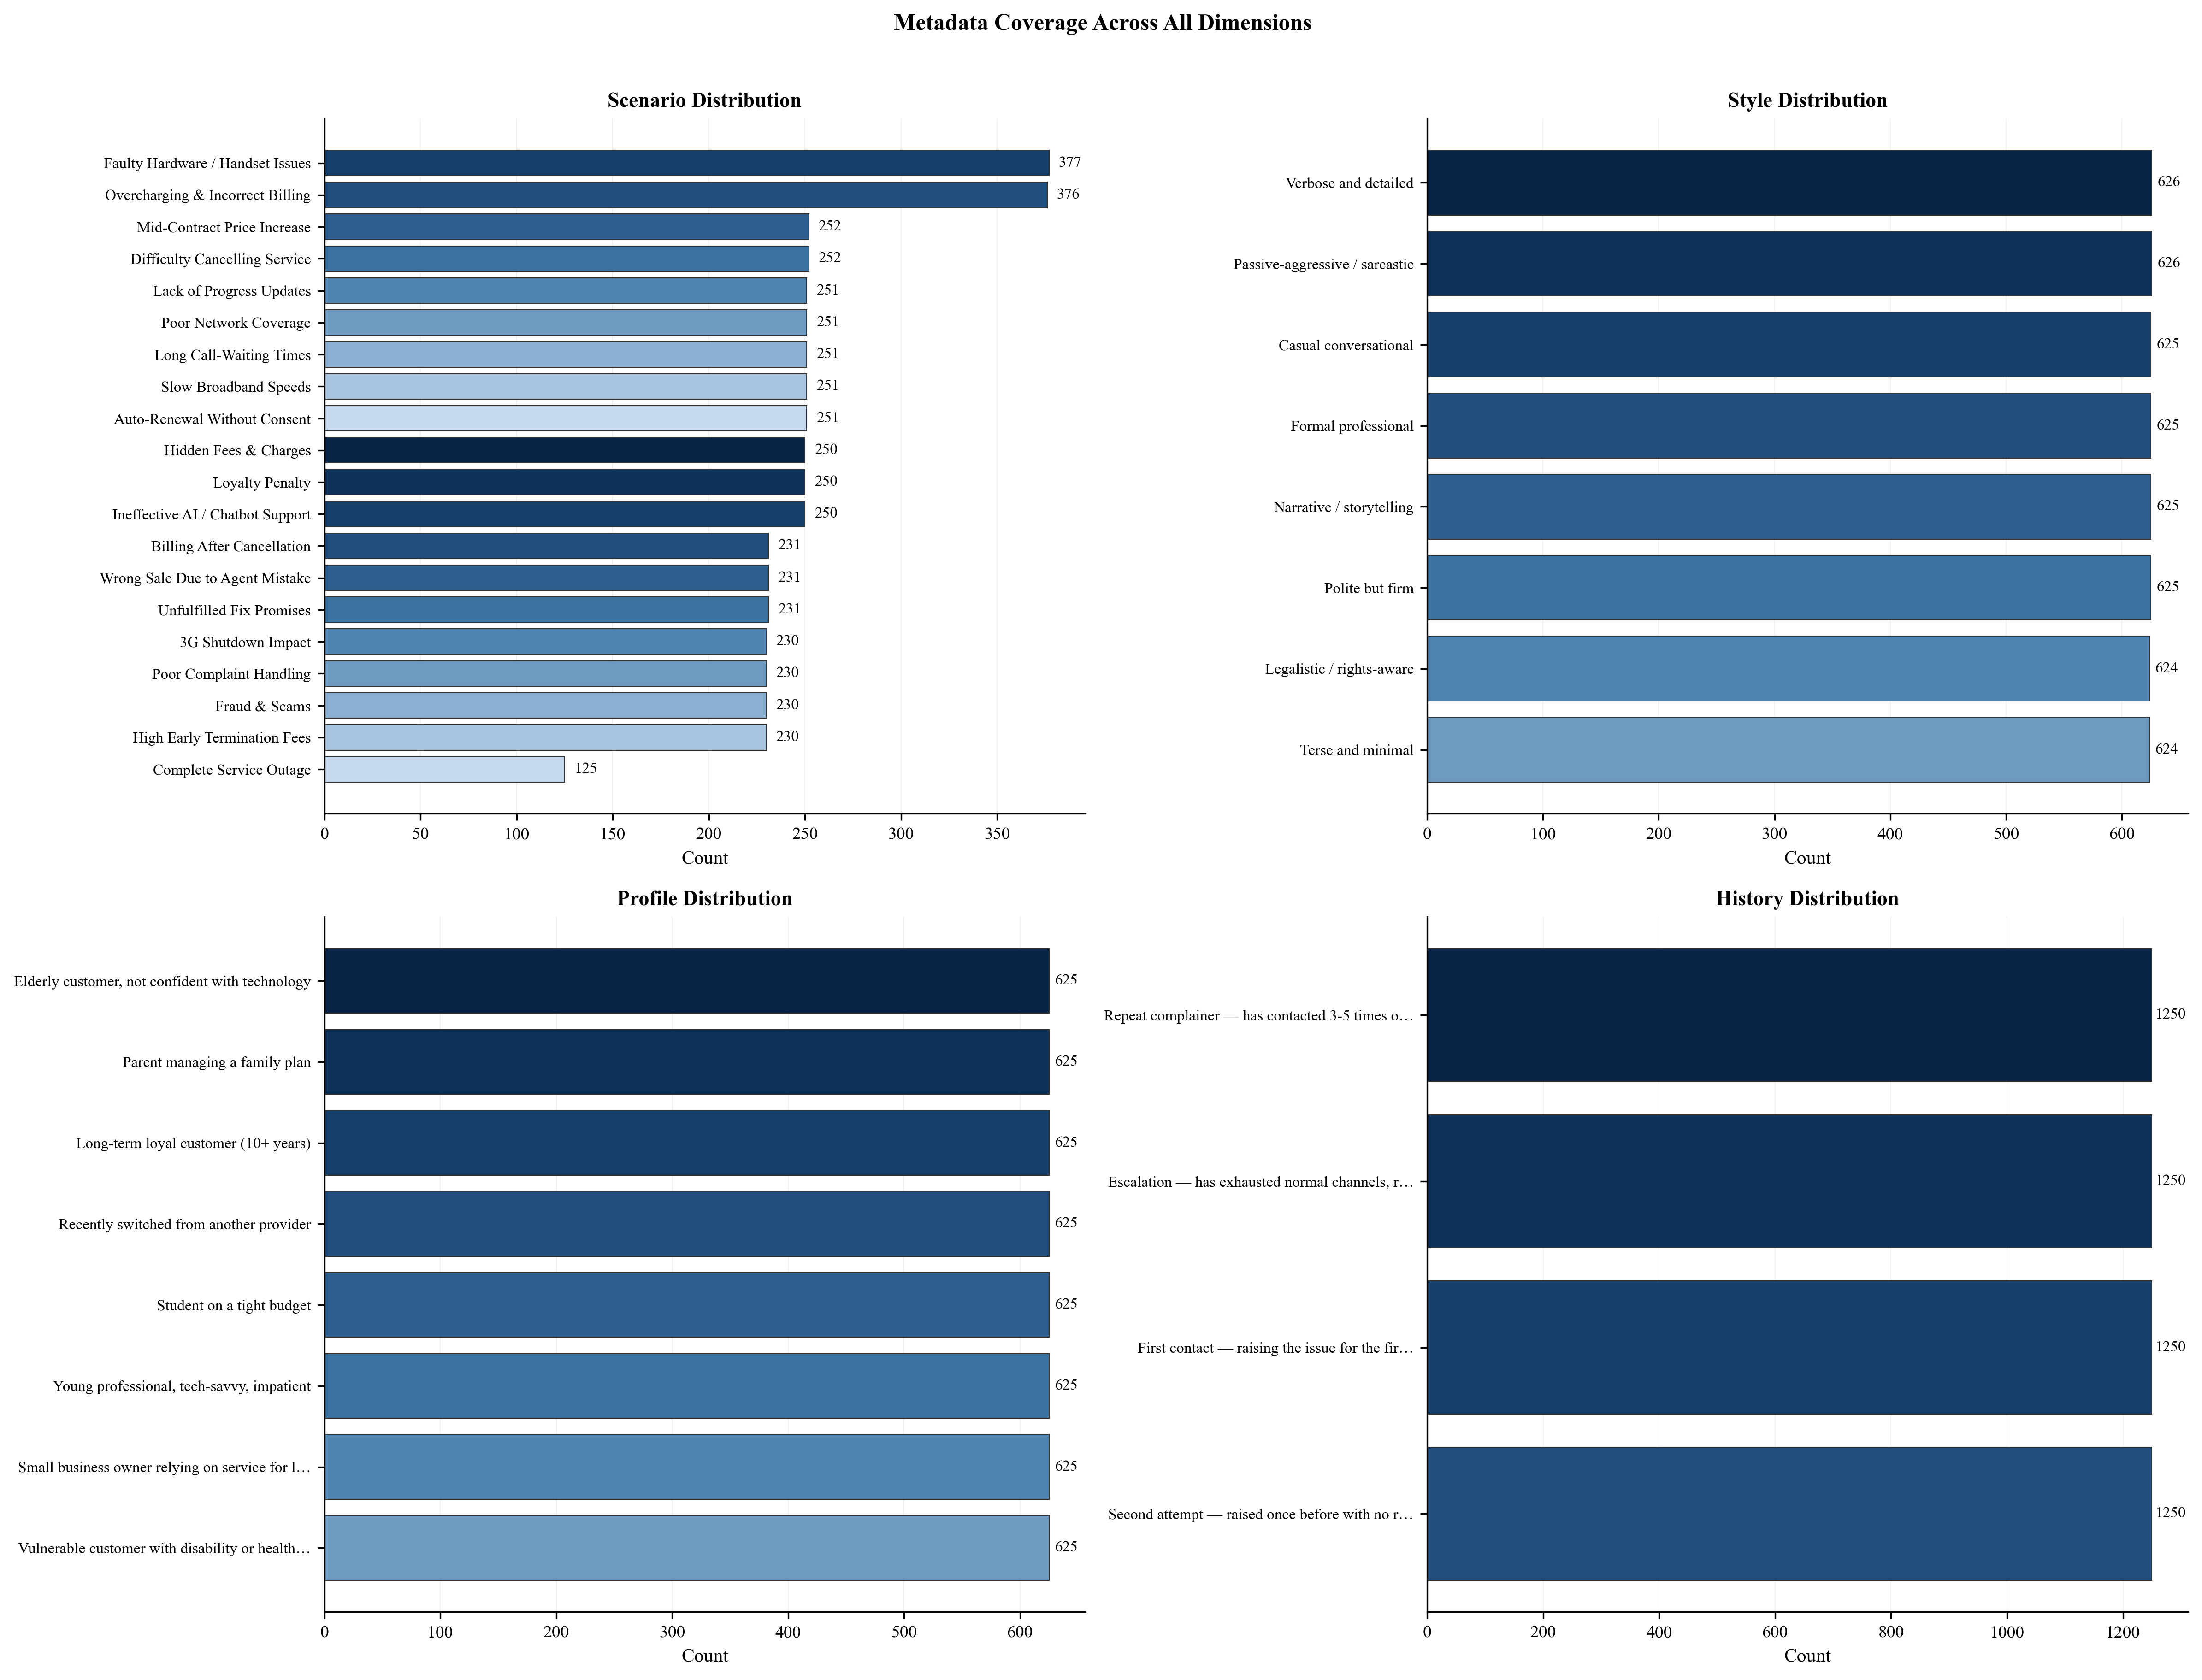
\includegraphics[width=\textwidth]{figures/fig09_metadata_coverage.png}
  \caption{Coverage of scenario, style, profile, and history attributes across the
  5,000-complaint synthetic dataset, demonstrating broad metadata distribution rather
  than concentration in any single category.}
  \label{fig:metadata}
\end{figure}

\section{Writing Style -- Emotion Independence}

\begin{figure}[H]
  \centering
  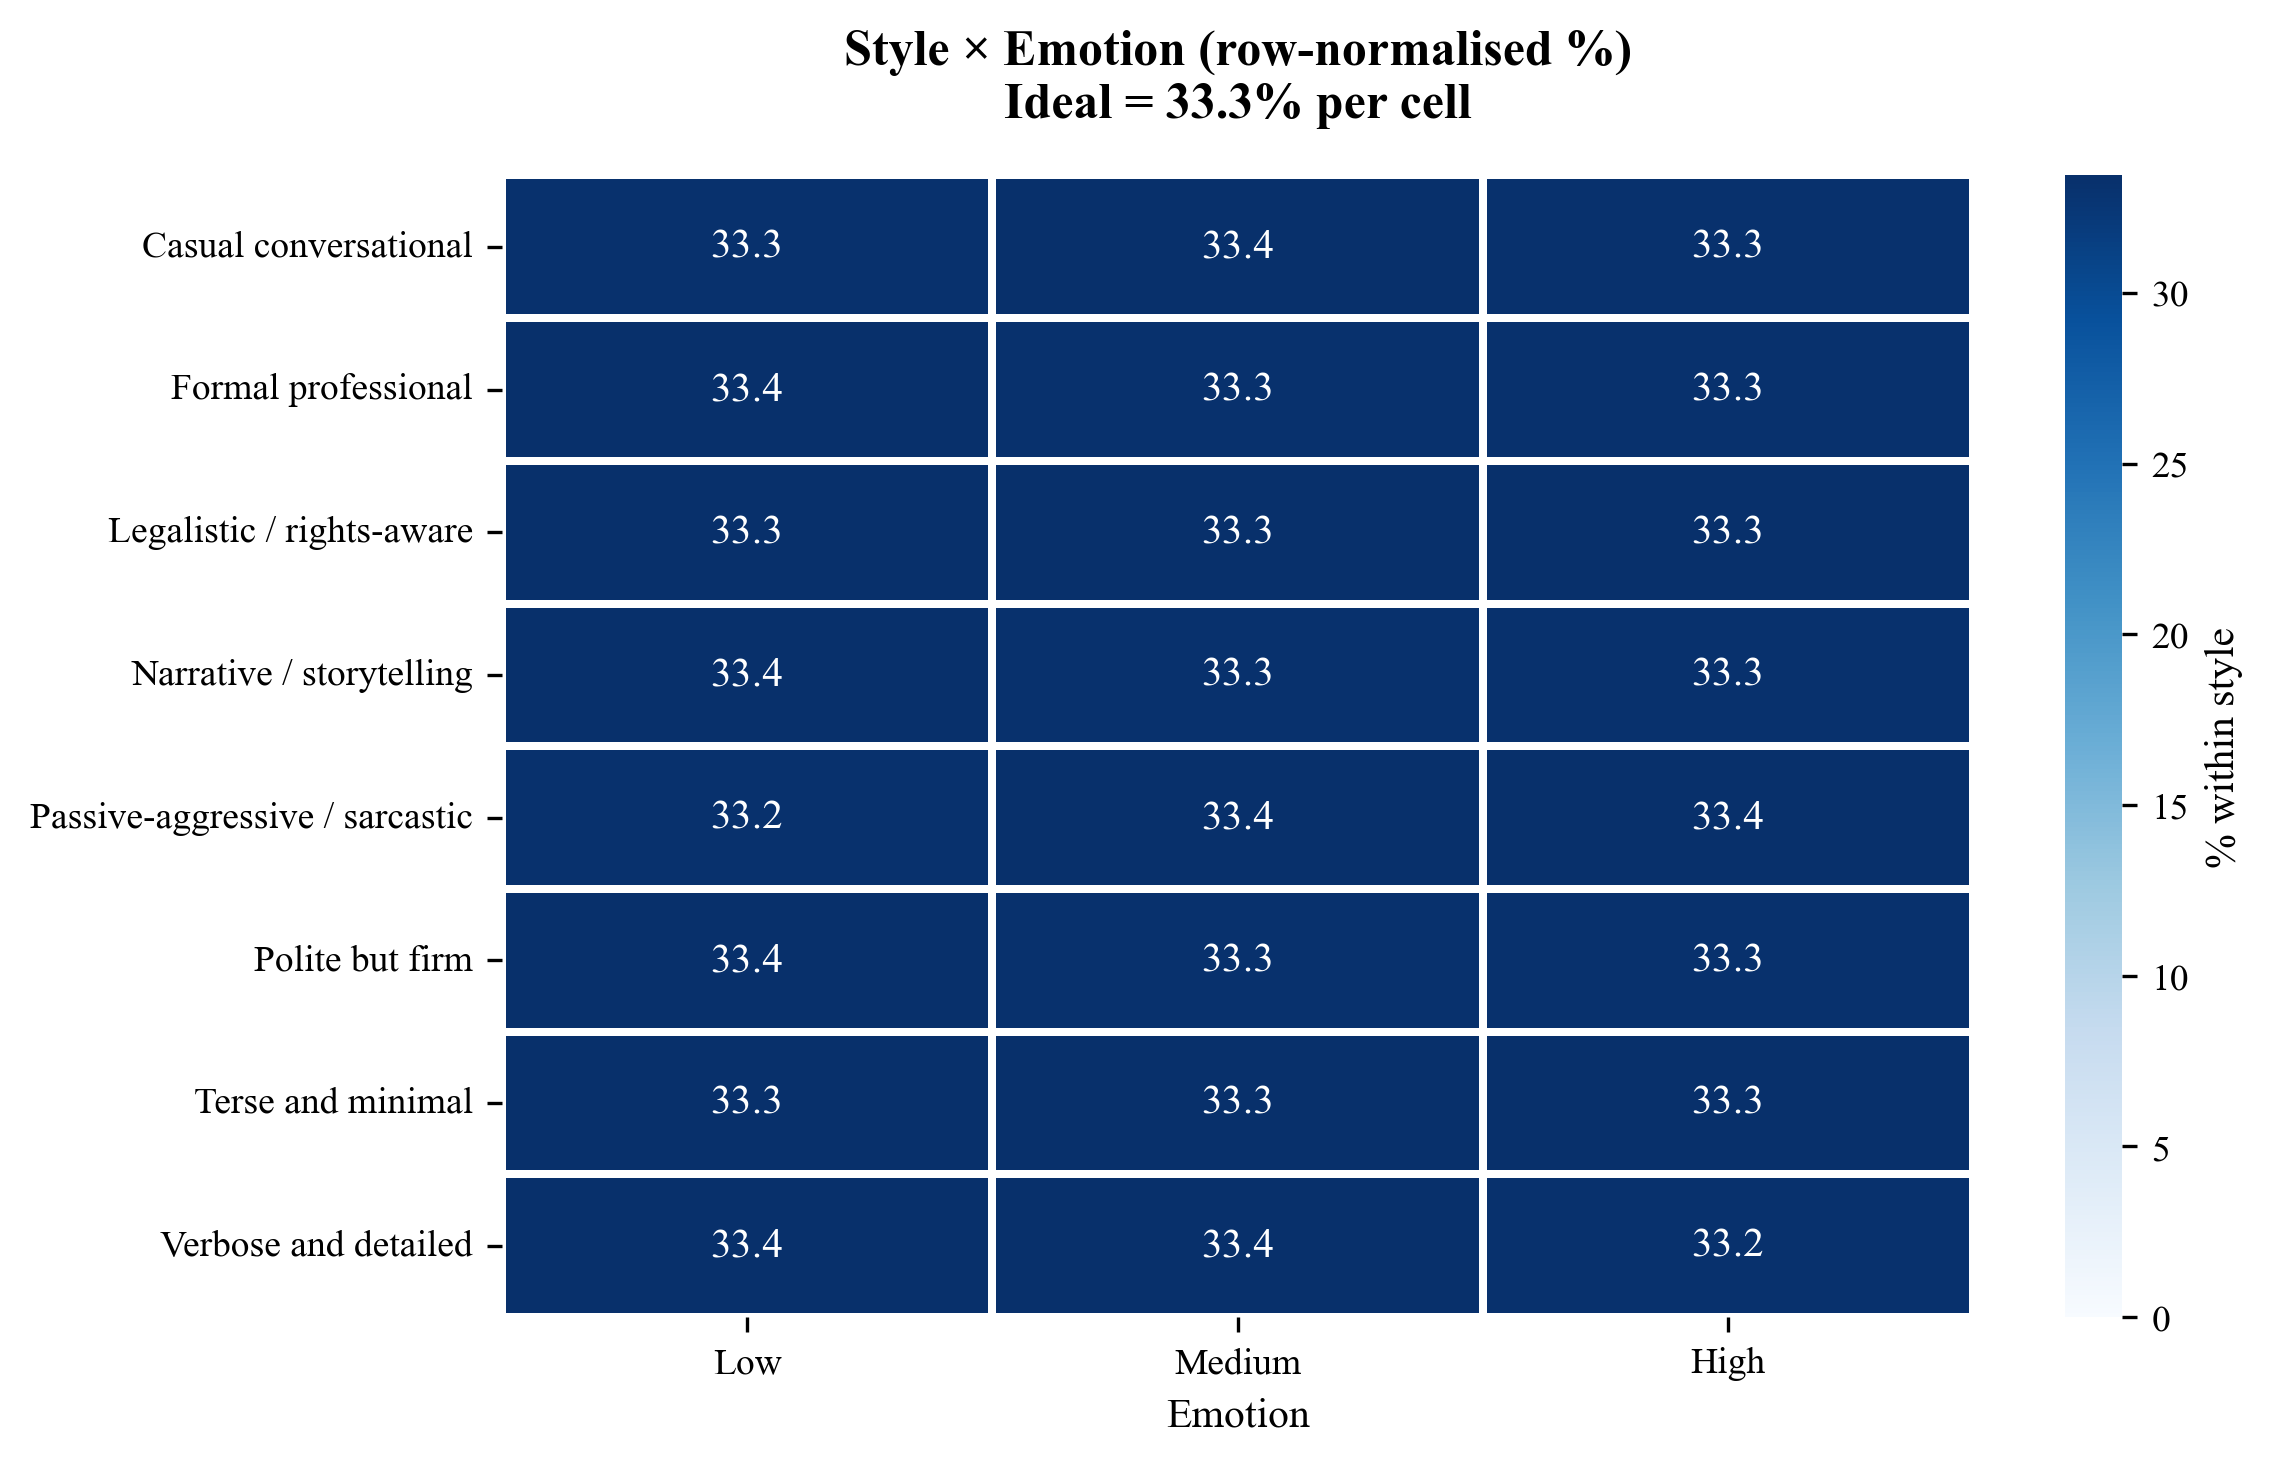
\includegraphics[width=\textwidth]{figures/fig10_style_emotion_independence.png}
  \caption{Writing style distribution across emotion intensity levels, demonstrating
  that all styles appear at all emotion levels (no style-to-emotion leakage).}
  \label{fig:style_emotion}
\end{figure}

\section{Text Length and Token Truncation}

\begin{figure}[H]
  \centering
  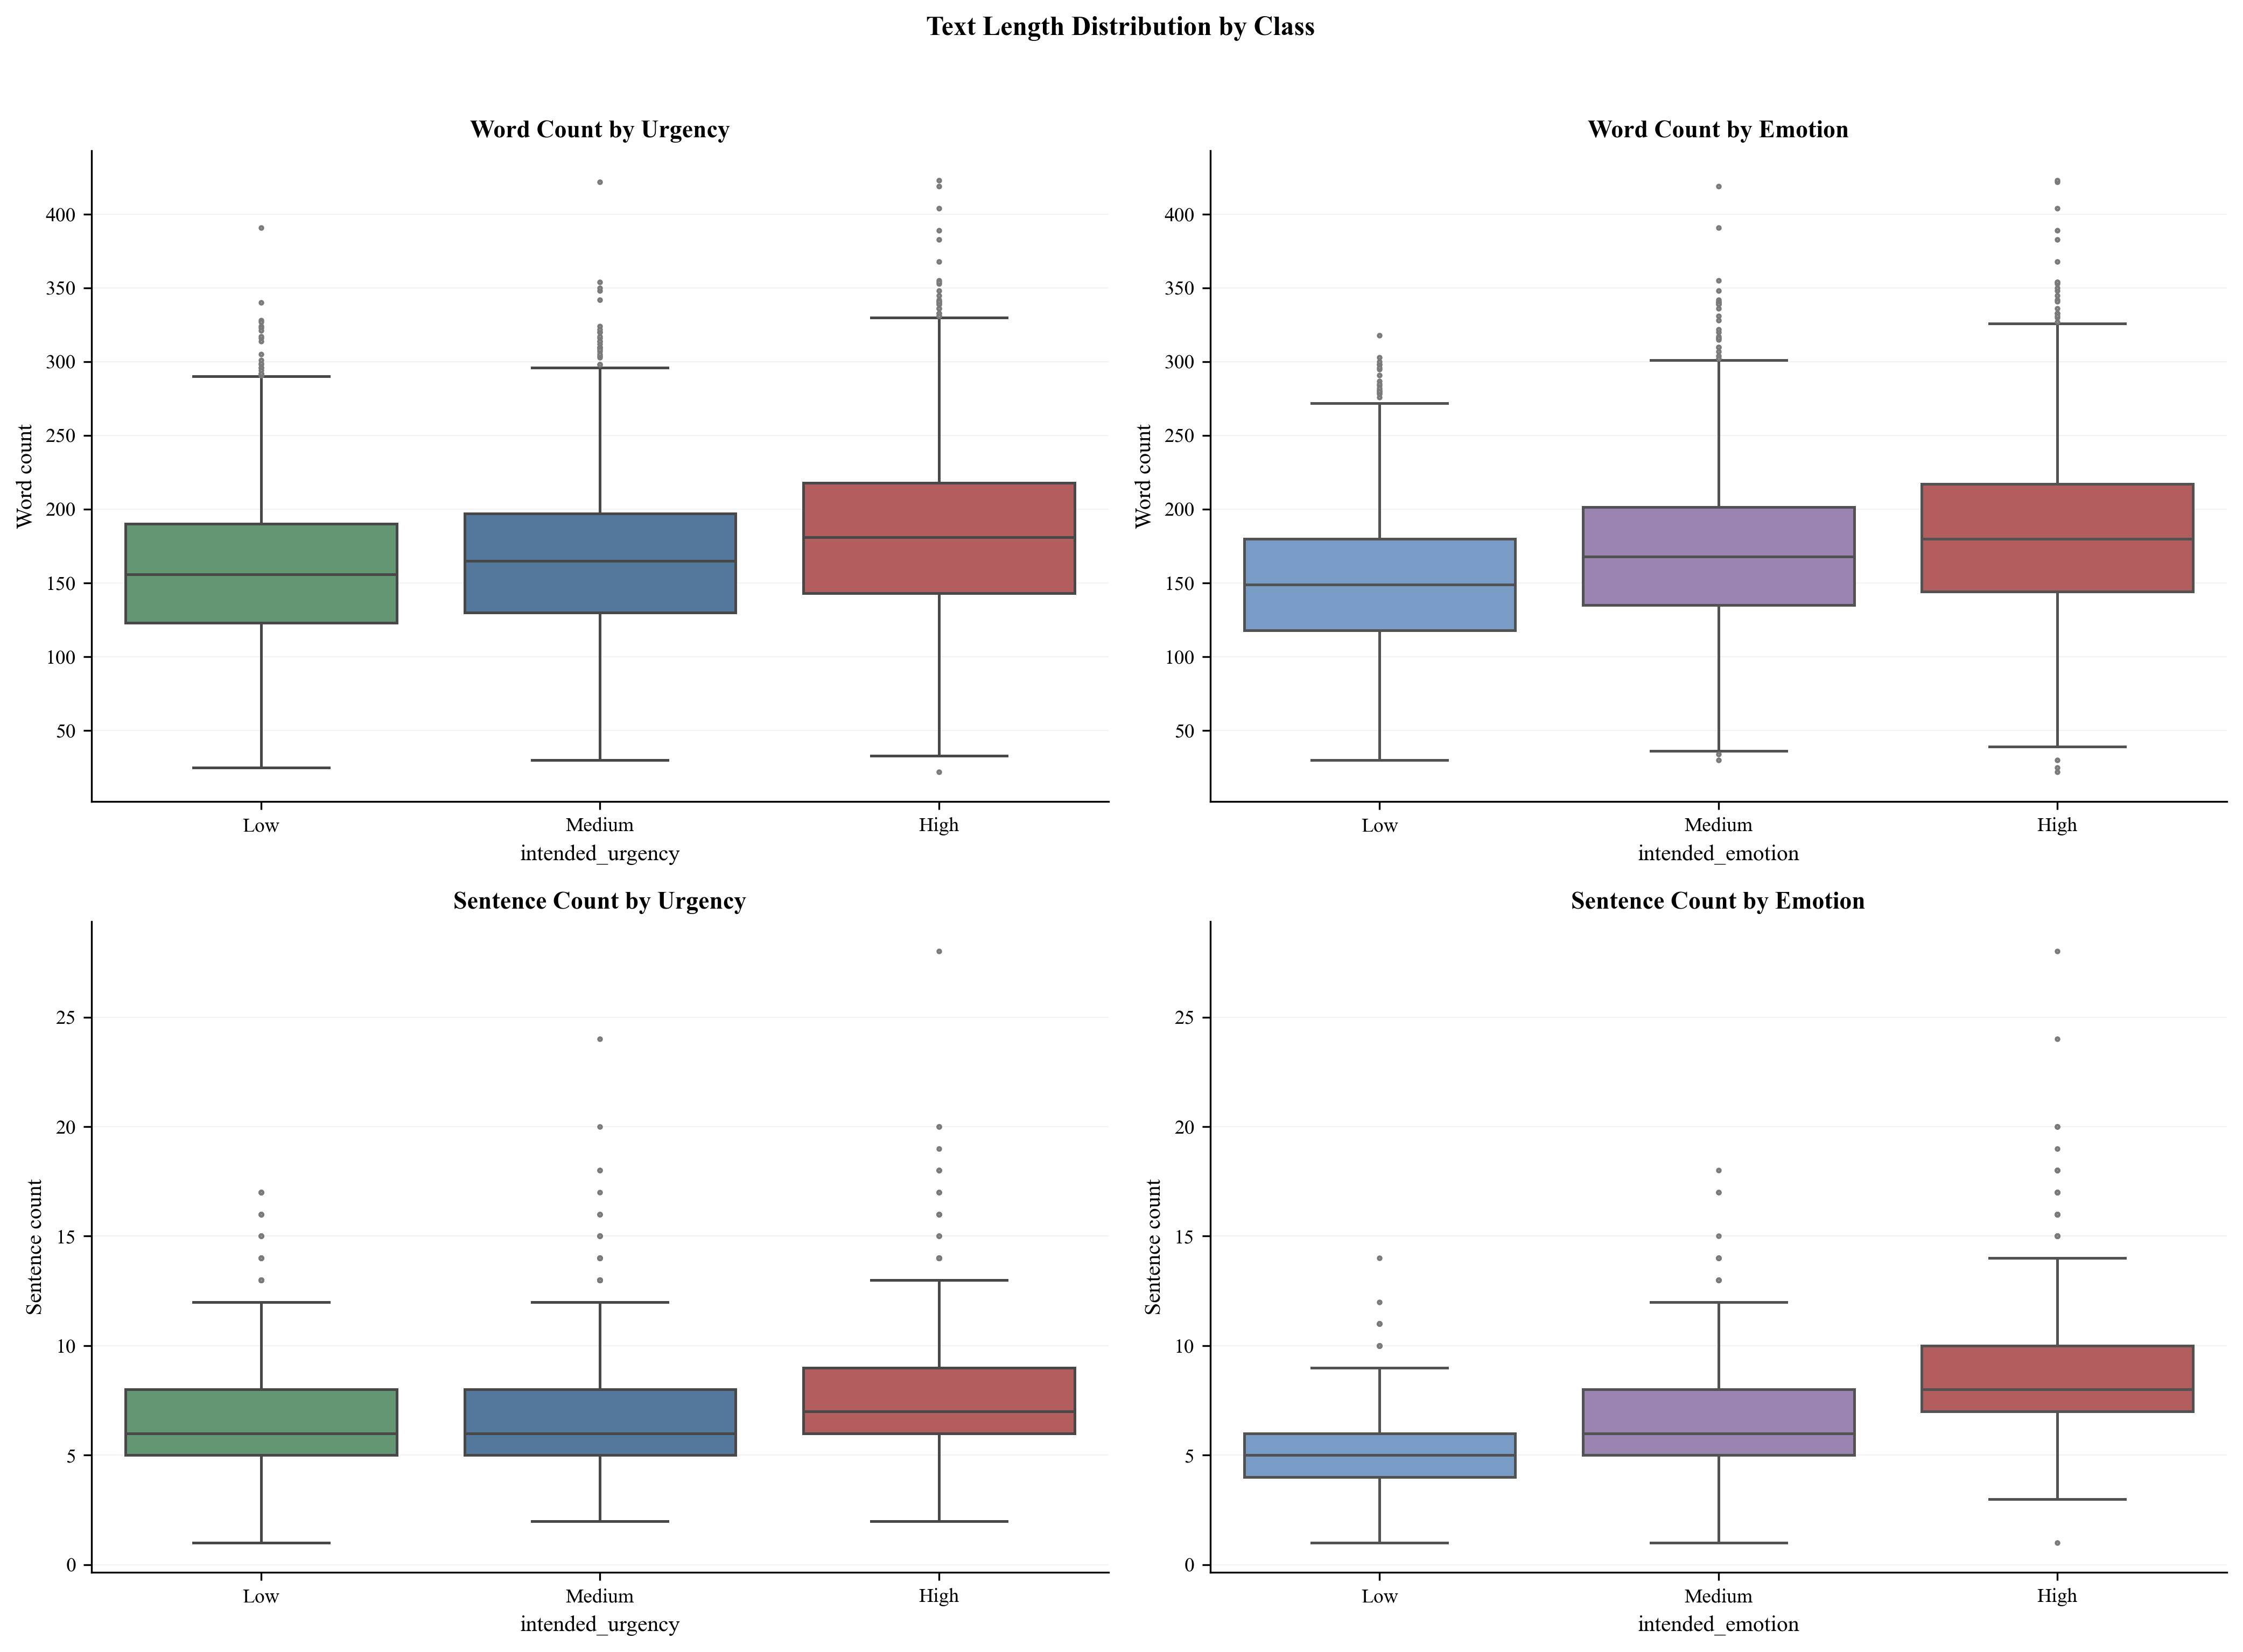
\includegraphics[width=\textwidth]{figures/fig11_text_length.png}
  \caption{Text length distribution by urgency and emotion class.}
  \label{fig:text_length}
\end{figure}

\begin{figure}[H]
  \centering
  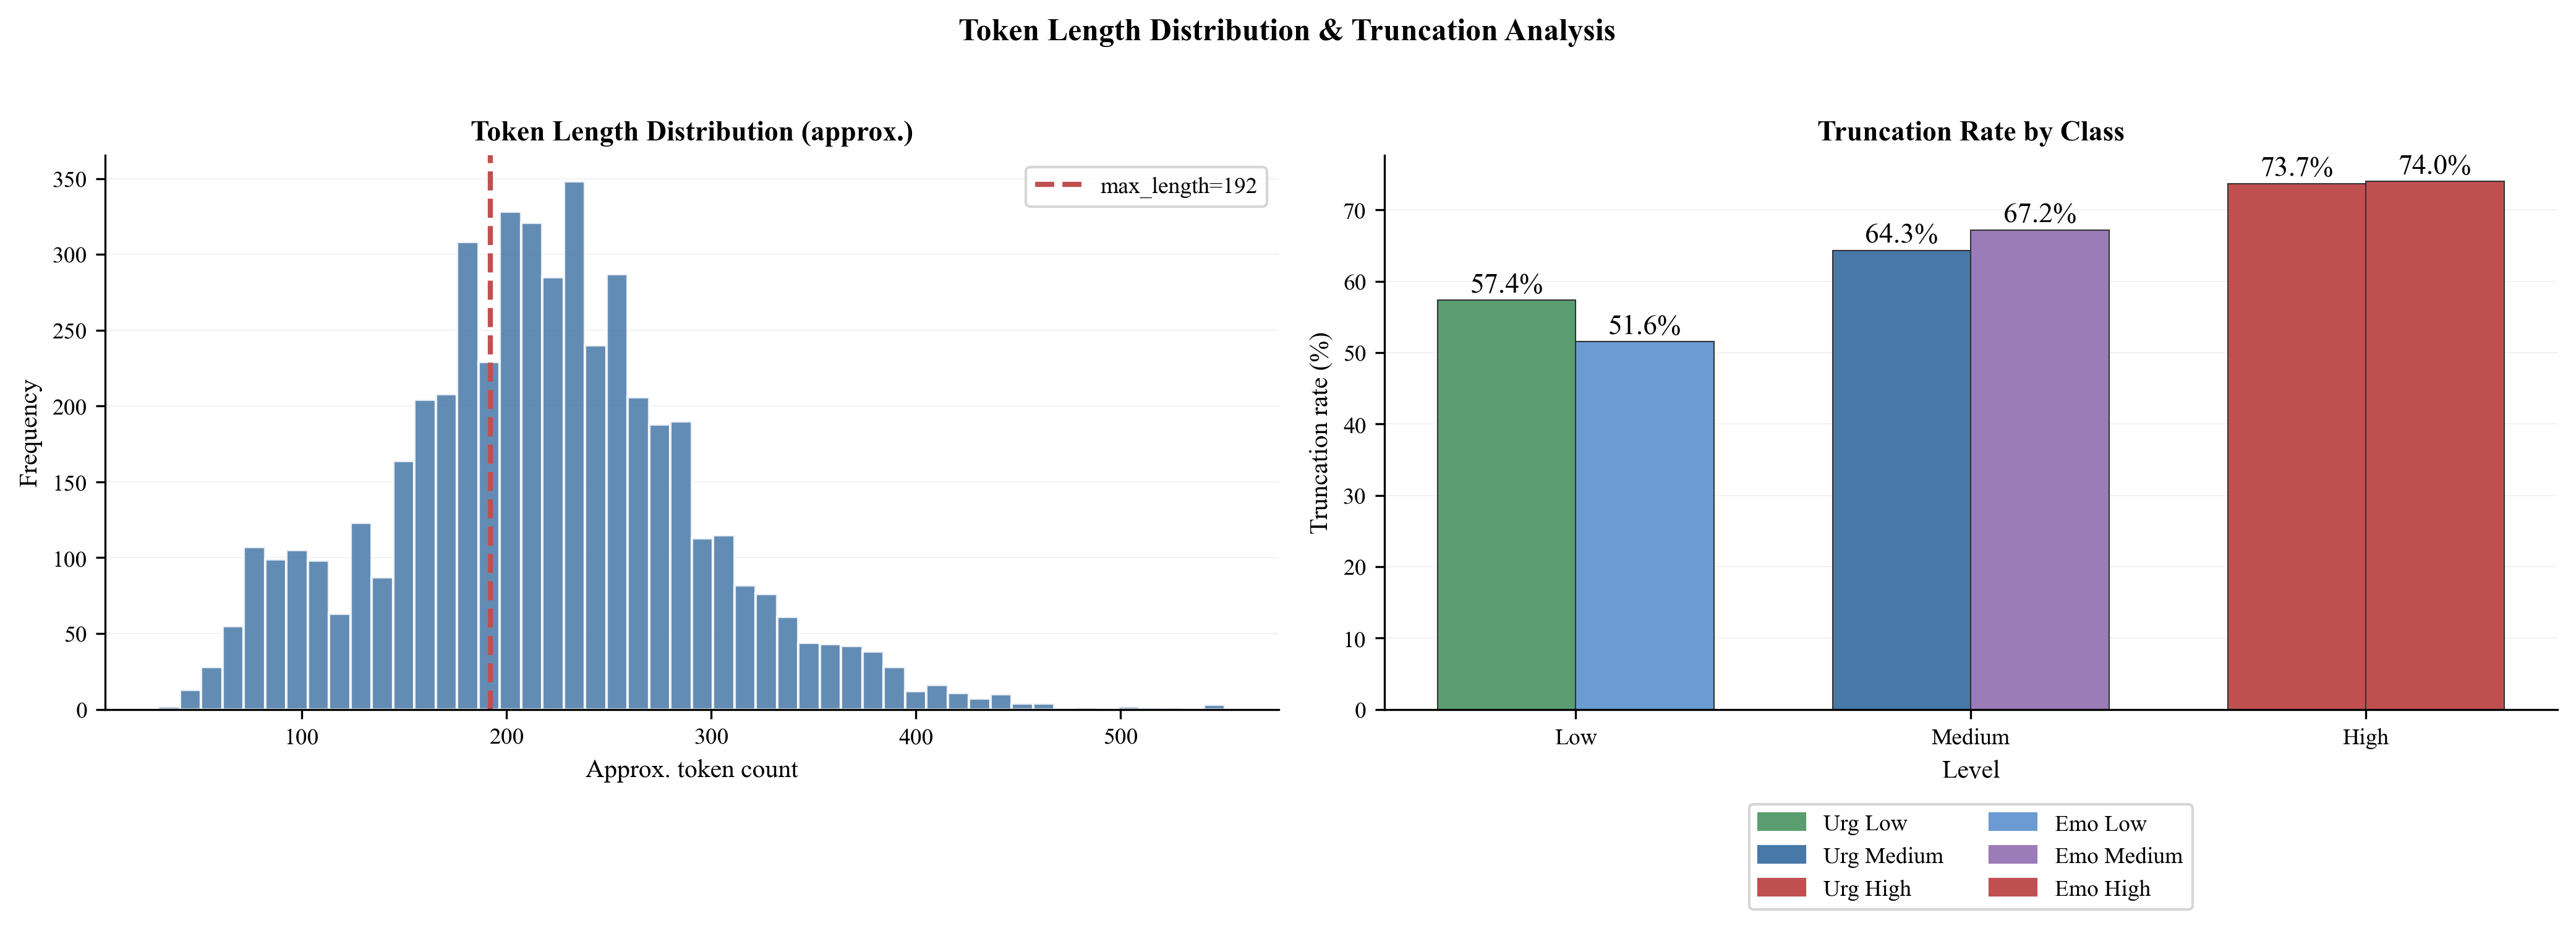
\includegraphics[width=\textwidth]{figures/fig12_token_truncation.png}
  \caption{Token truncation analysis at the 192-token sequence length limit.}
  \label{fig:token_trunc}
\end{figure}

\end{document}
